\documentclass{article} % For LaTeX2e
\usepackage{iclr2016_conference,times}
\usepackage{hyperref}
\usepackage{url}
\usepackage{graphicx}
%\usepackage[outdir=./]{epstopdf}
\usepackage[cmex10]{amsmath}
\usepackage{array}
\usepackage{mdwmath}
\usepackage{mdwtab}
\usepackage{eqparbox}
\usepackage{tikz}
\usepackage{tikz-qtree}
\usepackage{stfloats}
\hyphenation{net-works Boltz-mann}
\usepackage{times}
\usepackage{xcolor}
\usepackage{amssymb}
\usepackage{epsfig}
\usepackage{amssymb}
\usepackage[]{algorithm2e}
\usepackage{floatrow}
% Table float box with bottom caption, box width adjusted to content
%\usepackage{capt-of}
%\usepackage[normalem]{ulem}
% \usepackage[all=normal,floats=tight,paragraphs=tight,indent=tight]{savetrees}
% \usepackage[subtle]{savetrees}

% \renewcommand{\baselinestretch}{0.97}

\newcommand{\argmax}{\arg\!\max}
\definecolor{green}{rgb}{0.2,0.8,0.2}
\definecolor{blue}{rgb}{0.2,0.2,0.8}
\usepackage{xspace}
\newcommand*{\eg}{e.g.\@\xspace}
\newcommand*{\ie}{i.e.\@\xspace}
\newcommand*{\aka}{a.k.a.\@\xspace}
\makeatletter
\newcommand*{\etc}{%
    \@ifnextchar{.}%
        {etc}%
        {etc.\@\xspace}%
}


\title{Sequence Level Training with\\Recurrent Neural Networks}


\author{Marc'Aurelio Ranzato, Sumit Chopra, Michael Auli, Wojciech Zaremba \\
Facebook AI Research\\
\texttt{\{ranzato, spchopra, michealauli, wojciech\}@fb.com}
}

% The \author macro works with any number of authors. There are two commands
% used to separate the names and addresses of multiple authors: \And and \AND.
%
% Using \And between authors leaves it to \LaTeX{} to determine where to break
% the lines. Using \AND forces a linebreak at that point. So, if \LaTeX{}
% puts 3 of 4 authors names on the first line, and the last on the second
% line, try using \AND instead of \And before the third author name.

\newcommand{\fix}{\marginpar{FIX}}
\newcommand{\new}{\marginpar{NEW}}
\newcommand{\bh}{\mathbf{h}}
\newcommand{\bb}{\mathbf{b}}
\newcommand{\bx}{\mathbf{x}}
\newcommand{\bc}{\mathbf{c}}
\newcommand{\bone}{\mathbf{1}}
\newcommand{\by}{\mathbf{y}}
\newcommand{\bs}{\mathbf{s}}
\newcommand{\btheta}{\mathbf{\theta}}
\newcommand{\bo}{\mathbf{o}}
\newcommand{\setr}{\mathcal{R}}
\newcommand{\mamark}[1]{\textcolor{orange}{{#1}}}
\newcommand{\spcmark}[1]{\textcolor{red}{{#1}}}
\newcommand{\macomment}[1]{\marginpar{\begin{center}\textcolor{orange}{#1}\end{center}}}
\iclrfinalcopy % Uncomment for camera-ready version



\begin{document}
\maketitle

%\baselinestretch{0.95}

\begin{abstract}
Many natural language processing applications use language models to generate text.
These models are typically trained to predict the next word in a sequence, given the previous words and some context such as an image. 
However, at test time the model is expected to generate the entire sequence from scratch. 
This discrepancy makes generation brittle, as errors may accumulate along the way. 
We address this issue by proposing a novel sequence level training algorithm that directly optimizes the metric used at test time, such as BLEU or ROUGE.
On three different tasks, our approach outperforms several strong baselines for greedy generation. The method is also competitive when these baselines employ beam search,
 while being several times faster. 
\end{abstract}

\section{Introduction}

Locating visual landmarks, such as human body joints \cite{toshev2014deeppose} and facial key points \cite{xiong2013supervised}, is an important yet challenging problem. The stacked U-Nets, {\it e.g.} hourglasses (HGs) \cite{newell2016stacked}, are widely used in landmark localization. Generally speaking, their success can be attributed to design patterns: 1) within each U-Net, connect the top-down and bottom-up feature blocks to encourage gradient flow; and 2) stack multiple U-Nets in a cascade to refine prediction stage by stage.

However, the shortcut connection exists only ``locally'' inside each U-Net \cite{ronneberger2015u}. There is no ``global'' connection across U-Nets except the cascade. Blocks in different U-Nets cannot share features, which may impede the information flow and lead to redundant parameters.

We propose densely connected U-Nets (DU-Net) to address this issue. The key idea is to directly connect blocks of the same semantic meanings, {\it i.e.} having the same resolution in either top-down or bottom-up context, from any U-Net to all subsequent U-Nets. Please refer to Fig. \ref{fig:framework} for an illustration. The dense connectivity is similar to DenseNet \cite{huang2016densely} but generalizing the design philosophy from feature to semantic level. It encourages information flow as well as feature reuse ``globally'' across the stacked U-Nets, yielding improved localization accuracy. 

Yet there are critical issues in designing DU-Net: 1) The number of parameters would have a quadratic growth since $n$ stacked U-Nets could generate $O(n^2)$ connections. 2) A naive implementation may allocate new memory for every connection, making the training highly expensive and limiting the maximum depth of DU-Nets. 

% The training would be extremely memory expensive since a naive implementation has to make a copy of every connected feature for network forward and back propagation.  



\begin{figure*}[t!]
\centering
  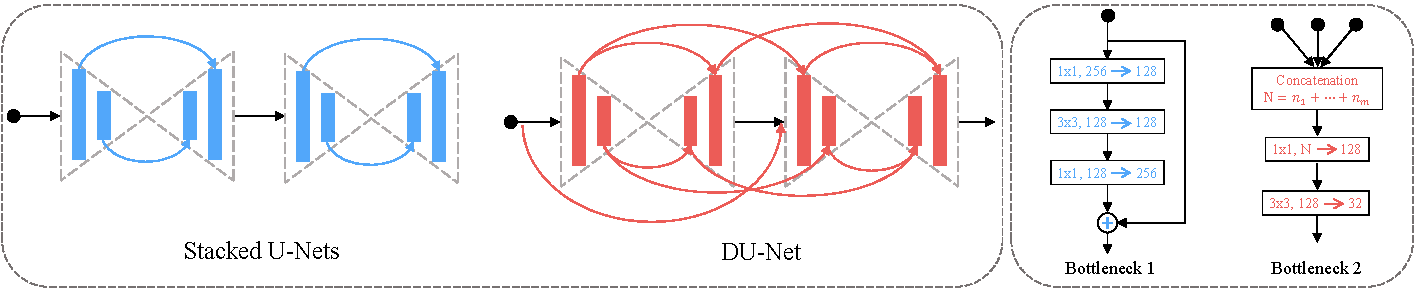
\includegraphics[width=1.0\linewidth]{figures/framework-cropped.pdf}
\caption{Illustration of stacked U-Nets and DU-Net. Stacked U-Nets has skip connections only within each U-Net. In contrast, DU-Net also connects blocks with the same semantic meanings across different U-Nets. The feature reuse could significantly reduce the size of bottleneck in each block, as shown in the right figure. Consequently, with the same number of U-Nets, DU-Net has only 30\% parameters of stacked U-Nets.}
\label{fig:framework}
\end{figure*}

% 
Our solution to those efficiency issues is threefold. {\bf First}, instead of connecting all stacked U-Nets, we only connect a U-Net to its $K$ successors. We name it as the $order$-$K$ connectivity, which aims to balance the fitting accuracy and parameter efficiency by cutting off long-distance connections. {\bf Second}, we employ a memory-efficient implementation in training. The key idea is to reuse a pre-allocated memory so all connected blocks could share the same memory. Compared with the naive implementation, this strategy makes it possible to train a very deep DU-Net (actually, $2\times$ deeper). {\bf Third}, to further improve the efficiency, we investigate an iterative design that may reduce the model size to one half. More specifically, the output of the first pass of the DU-Net is used as the input of the second pass, where detection or regression loss is applied as supervision. 

% %G%
% In view of deploying our approach on mobile devices, we further attempt to quantize weights, inputs, and gradients of DU-Net to low bit-width discrete values. This not only decreases the high precision operations but also shrinks the memory usage during training. By network quantization, the size of trained model can also be largely compressed.
% %G%
Besides shrinking the number of network parameters, we also study to further quantize each parameter. This motivates from the ubiquitous mobile applications. Although current mobile devices could carry models of dozens of MBs, deploying such networks requires high-end GPUs. However, quantized models could be accelerated by some specifically designed low-cost hardwares. Beyond only deploying models on mobile devices \cite{li2017deeprebirth}, training deep neural networks on distributed mobile devices emerges recently \cite{mcmahan2016communication}. To this end, we also try to quantize not only the model parameters but also its inputs (intermediate features) and gradients in training. This is the first attempt to investigate training landmark localizers using quantized inputs and gradients.


In summary, our key contributions are:
\begin{itemize}
    \item To the best of our knowledge, we are the first to propose quantized densely connected U-Nets for visual landmark localization, which largely improves the information flow and feature reuse at the semantic level.
    \item We propose the $order$-$K$ connectivity to balance accuracy and efficiency. It decreases the growth of model size from quadratic to linear by removing trivial connections. Experiments show it could reduce $\sim$70\% parameters of state-of-the-art landmark localizers.
    \item Very deep U-Nets can be trained using a memory-efficient implementation, where pre-allocated memory is reused by all connected blocks.
    \item We further investigate an iterative refinement that may cut down half of the model size, by forwarding DU-Net twice using either detection or regression supervision.
    %G%
    \item Different from previous efforts of quantizing only the model parameters, we are the first to quantize their inputs and gradients for better training efficiency on landmark localization tasks. By choosing appropriate quantization bit-widths for weights, inputs and gradients, quantized DU-Net achieves $\sim$75\% training memory saving with comparable performance. 
    %G%
    \item Exhaustive experiments are performed to validate DU-Net in different aspects. In both human pose estimation and face alignment, DU-Net demonstrates comparable localization accuracy and use $\sim$2\% model size compared with state-of-the-art methods.
\end{itemize}

% We are the first to deploy network quantization for better training efficiency on localization tasks. By choosing appropriate quantization bit-widths for weights, inputs and gradients, quantized DU-Net achieves at least 32$\times$ memory saving with comparable performance to the-state-of-art approaches. 


%The landmark localization such as human pose estimation \cite{toshev2014deeppose,newell2016stacked,wei2016convolutional}, facial landmark localization \cite{xiong2013supervised,zhang2014facial,sagonas2013300}, etc, plays an important role in the higher-level image understanding. The Convolutional Neural Networks (CNNs) have dominated this field, among which recent architecture of stacked hourglasses \cite{newell2016stacked}, a variant of the U-Net \cite{ronneberger2015unet}, becomes a standard solution. The skip connections between top-down and bottom-up blocks within a U-Net could preserve the spatial information and increase the gradient flow. With multiple U-Nets stacked together, the prediction could be refined stage by stage. However, the connections are only within each U-Net of the stacked hourglasses and no explicit connections exist between U-Nets, which may impede the information flow across them. And the blocks with the same semantics in different U-Nets cannot share features, leading to many redundant parameters. 

% Its success attributes to three key factors: repeated top-down, bottom-up inferences, intermediate supervisions and residual bottlenecks \cite{}. 

% The multiple stage top-down and bottom-up processing could better integrate both the local and global visual contexts into the final prediction. The intermediate supervision and residual bottlenecks, on the other hand, could alleviate the gradient vanish problem in deep networks.
%In this paper, we propose to densely connect stacked U-Nets by linking blocks with the same semantics in different U-Nets. We refer to this architecture as {\it Dense U-Nets}. The blocks in a U-Net could get direct inputs from its connected blocks in all preceding U-Nets, making the information flow more efficiently among the U-Nets. The feature reuse at each resolution could reduce the parameters in each block. The dense connectivity in our Dense U-Nets is different from that of DenseNet \cite{huang2016densely}. More specifically, layers only within each single block of the DenseNet are connected. In contrast, we connect blocks lying across the whole Dense U-Nets and connections of hierarchical blocks are mixed together. An illustration is given in Figure \ref{fig:framework}. We name it as the {\it global dense connectivity} to differentiate from the local one in the DenseNet.

% Besides, features in the Dense U-Nets are fused by the concatenation which could facilitate the information flow compared with the summation operation in the stacked hourglasses.

% Although the dense connectivity in our Dense U-Nets is similar with that of DenseNet \cite{}, 
% More recently, the DenseNet \cite{} achieves superior image classification performance over the ResNet \cite{} in terms of both the accuracy and model size, which benefits from the dense connections between layers. Its key insight is the feature reuse between layers of the same resolutions. The dense connectivity in the DenseNet, existing within one block, is local. By extending this principle, we propose a global dense connectivity, in contrast to the local connectivity in \cite{}, that blocks at the same locations of different U-Nets are connected. Hence, we refer to this architecture as {\it Dense U-Nets}. To our best knowledge, we are the first to generalize the local dense connectivity into the stacked U-Nets. 
% The global dense connectivity could make it easier to train much deeper stacked U-Nets.

% This motivates us to replace the residual modules  in the stacked hourglasses with the dense connected layers. However, this dense connectivity exists only locally within a contiguous  block in which all feature maps have the same spatial resolution. A U-Net, on the other hand, consists of a sequence of top-down and bottom-up blocks. A straight way is to turn each block into a dense block with multiple layers. However, this would sacrifice the spirit of stacked hourglasses that multiple stacked hourglasses outperform a single hourglass with multiple layers in each block.

% In order to integrate the structure of stacked U-Nets together with the idea of dense connectivity, we propose a global dense connectivity, in contrast to the local connectivity in \cite{}, that blocks at the same locations of different U-Nets are connected. Hence, we refer to this architecture as {\it Dense U-Nets}. The connected layers in the Dense U-Nets distribute along the whole network rather than in local continuous blocks. Compared with the local residual modules in the stacked hourglasses, the global dense connections could significantly facilitate the gradient to flow across stacked U-Nets.

%In practice, the Dense U-Nets have the efficiency problems of both parameter and training memory. First, suppose a Dense U-Nets contains $n$ U-Nets, there would be $O(n(n-1)/2)$ connections. Even though we use the dense bottleneck in Figure \ref{fig:framework}, the number of conv($1\times 1$) parameters still has the quadratic growth. Inspired from the Variable Order Markov (VOM) models \cite{begleiter2004prediction}, we propose the order-K connectivity that, instead of linking all the U-Nets, we connect only a fixed number of U-Nets. The goal is to use the minimum connections achieving the most obvious improvements. The multiple intermediate supervisions in the Dense U-Nets are good compensates for the order-K connectivity since they could provide additional gradients. The DenseNet does not have this advantage since it has only one supervision at the end.

% Furthermore, different from the DenseNet with only one supervision, the Dense U-Nets have multiple intermediate supervisions. The global dense connections plus the intermediate supervisions could bring faster convergence on the training set, but also gives rise to the concern of overfitting. Inspired from the Variable Order Markov (VOM) models \cite{}, we propose the order-K connectivity that, instead of linking all the U-Nets, we connect only a fixed number of U-Nets. The goal is to use the minimum connections achieving the most obvious improvement. Another advantage of order-K connectivity is that it has fewer parameters compared with the dense connectivity.

%Benefiting from the order-K connectivity, the Dense U-Nets could achieve comparable performance of stacked hourglasses with only one-third parameters. However, a naive implementation of the order-K connectivity could make the training very memory expensive. Therefore, we employ the memory efficient implementation \cite{pleiss2017memory}. The key idea is to share memories for time efficient operations such as concatenation and batch norm \cite{ioffe2015batch} within the connected layers. By pre-allocating a fixed memory, the later features produced by these operations would replace earlier features. So we need to re-compute those replaced features in the backward phase. The memory efficient implementation makes it possible to train Dense U-Nets two times deeper than the stacked hourglasses. 

%Furthermore, we also investigate to use the iterative refinement improving the parameter efficiency. Given a Dense U-Nets, we compare its performance with another Dense U-Nets with only half depth but an additional iteration. Besides, both detection and regression losses \cite{bulat2016human} were used in the landmark detection tasks, but there is no investigation yet about how they independently and collaboratively affect the prediction. We will give their detailed comparison in our experiments.

%In summary, the key contributions are:
%\begin{itemize}
%    \item To our best knowledge, we are the first to use the dense connectivity among the stacked U-Nets. The global dense connectivity in our Dense U-Nets is different from the local one in the DenseNet \cite{huang2016densely}.
%    \item We propose the order-K connectivity to make the Dense U-Nets parameter efficient. The order-K connectivity could decrease the growth of conv($1\times 1$) parameters from quadratic to linear. With comparable performance as the stacked hourglasses \cite{newell2016stacked}, it makes the Dense U-Nets require only one-third parameters. 
%    \item The memory efficient implementation of Dense U-Nets is provided to reduce its training memory usage. It makes it possible to train Dense U-Nets two times deeper than the stacked hourglasses.
%    \item We further explore using iterative refinement to improvement the parameter efficiency. At the same time, we investigate how different combinations of the detection and regression losses affect the performance.
%\end{itemize}
\vspace{-0.09in}
\section{Model}
\label{sec:model}

Our non-parametric approach to solving one-shot learning is based on two components which we describe in the following subsections. First, our model architecture follows recent advances in neural networks augmented with memory (as discussed in Section~\ref{sec:relwork}). Given a (small) support set $S$, our model defines a function $c_S$ (or classifier) for each $S$, i.e. a mapping $S \rightarrow c_S(.)$. Second, we employ a training strategy which is tailored for one-shot learning from the support set $S$.

\vspace{-0.09in}
\subsection{Model Architecture}

\begin{figure}[t]
\centering
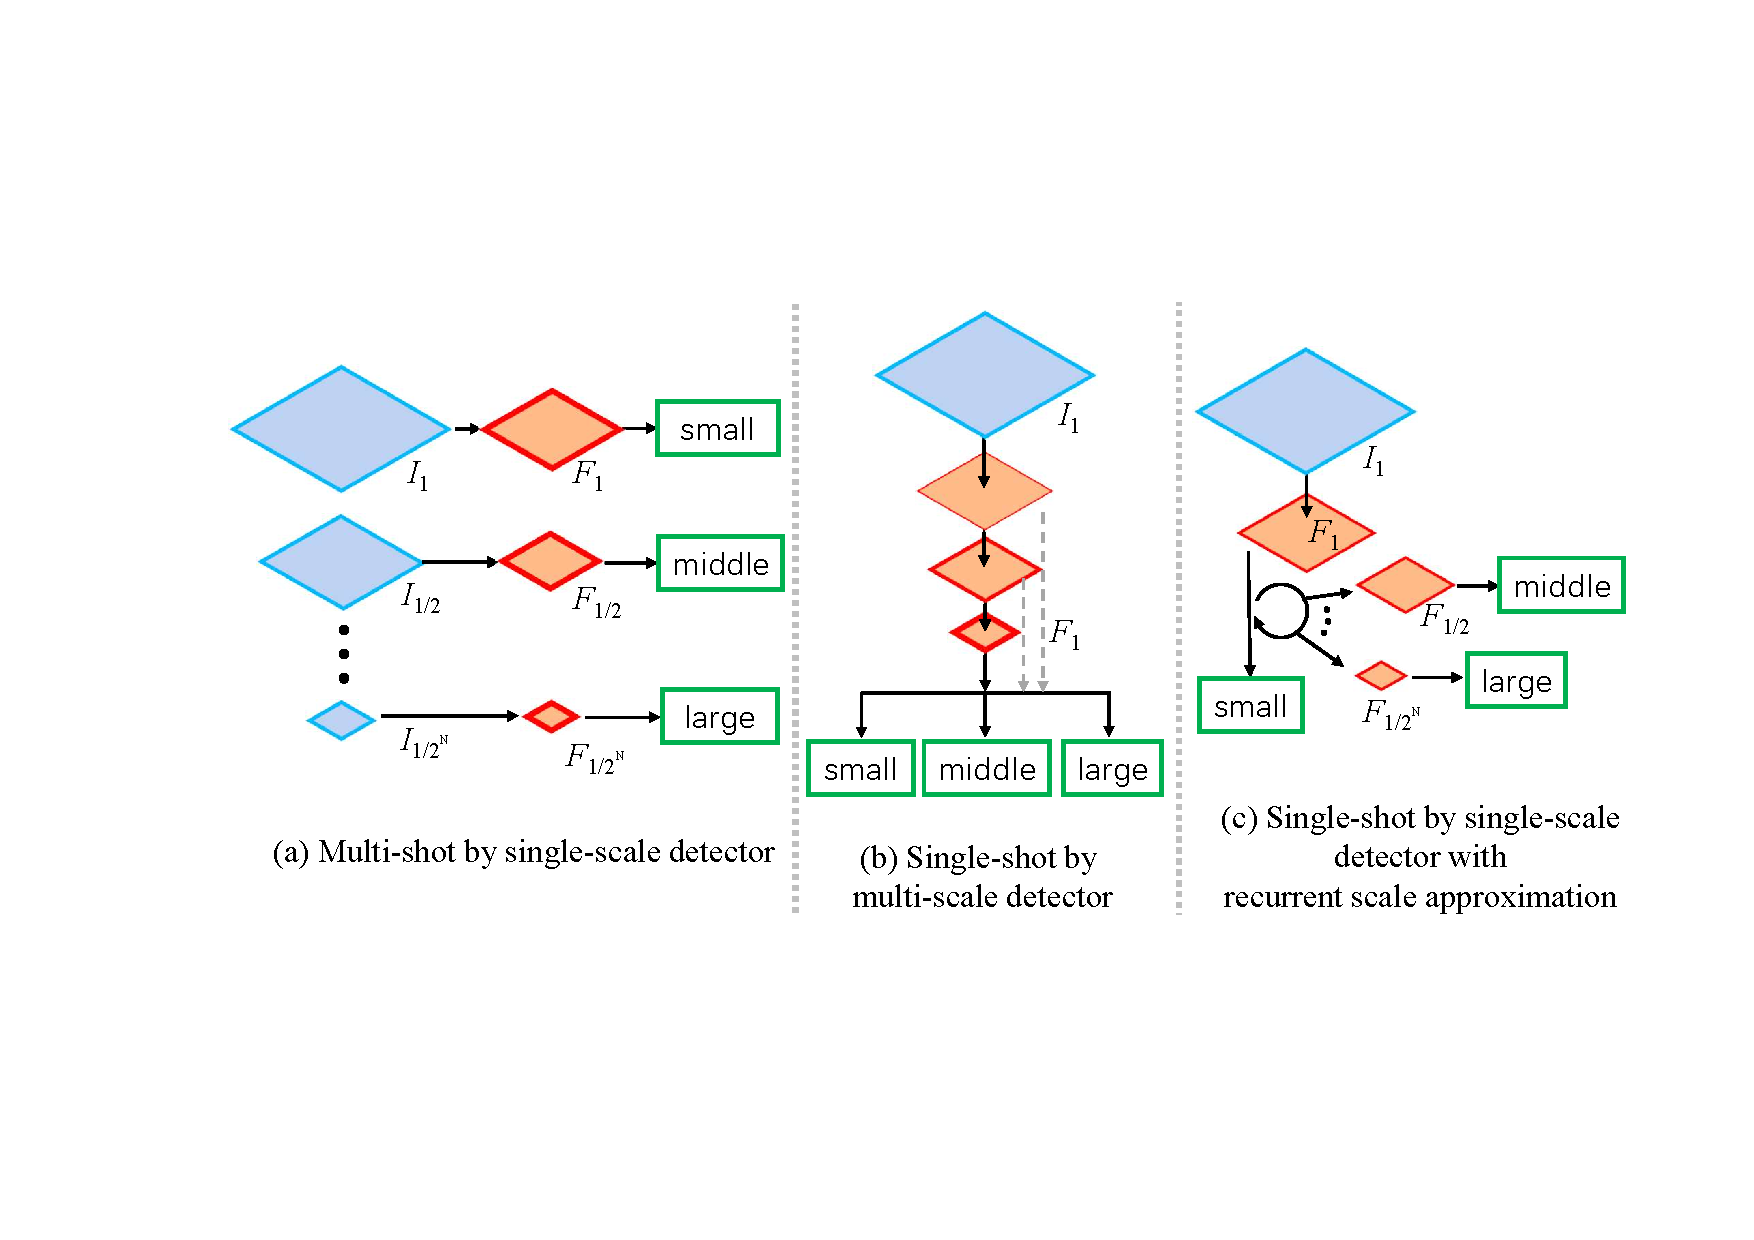
\includegraphics[width=.8\textwidth]{fig1}
\caption{\label{fig:arch}Matching Networks architecture}
\end{figure}

In recent years, many groups have investigated ways to augment neural network architectures with external memories and other components that make them more ``computer-like''. We draw inspiration from models such as sequence to sequence (seq2seq) with attention \cite{montreal}, memory networks \cite{memnets} and pointer networks \cite{ptrnets}.

In all these models, a neural attention mechanism, often fully differentiable, is defined to access (or read) a memory matrix which stores useful information to solve the task at hand. Typical uses of this include machine translation, speech recognition, or question answering. More generally, these architectures model $P(B|A)$ where $A$ and/or $B$ can be a sequence (like in seq2seq models), or, more interestingly for us, a set \cite{vinyals2015order}.

Our contribution is to cast the problem of one-shot learning within the set-to-set framework \cite{vinyals2015order}.
The key point is that when trained, Matching Networks are able to produce sensible test labels for unobserved classes \emph{without any changes to the network}.
More precisely, we wish to map from a (small) support set of $k$ examples of image-label pairs $S = \{(x_i, y_i)\}_{i=1}^k$ to a classifier $c_S(\hat{x})$ which, given a test example $\hat{x}$, defines a probability distribution over outputs $\hat{y}$.
We define the mapping $S\rightarrow c_S(\hat{x})$ to be $P(\hat{y} | \hat{x}, S)$ where $P$ is parameterised by a neural network. 
Thus, when given a new support set of examples $S'$ from which to one-shot learn, we simply use the parametric neural network defined by $P$ to make predictions about the appropriate label $\hat{y}$ for each test example $\hat{x}$: $P(\hat{y}|\hat{x}, S')$.
In general, our predicted output class for a given input unseen example $\hat{x}$ and a support set $S$ becomes $\arg\max_y P(y |\hat{x}, S)$.

Our model in its simplest form computes $\hat{y}$ as follows:

\begin{equation}
\hat{y} = \sum_{i=1}^{k} a(\hat{x},x_i) y_i
\label{eq:nn}
\end{equation}
where $x_i, y_i$ are the samples and labels from the support set $S=\{(x_i,y_i)\}_{i=1}^k$, and $a$ is an attention mechanism which we discuss below.
Note that eq.~\ref{eq:nn} essentially describes the output for a new class as a linear combination of the labels in the support set.
Where the attention mechanism $a$ is a kernel on $X\times X$, then \eqref{eq:nn} is akin to a kernel density estimator.
Where the attention mechanism is zero for the $b$ furthest $x_i$ from $\hat{x}$ according to some distance metric and an appropriate constant otherwise, then
\eqref{eq:nn} is equivalent to `$k-b$'-nearest neighbours (although this requires an extension to the attention mechanism that we describe in Section~\ref{sec:fce}).
Thus \eqref{eq:nn} subsumes both KDE and kNN methods.
Another view of \eqref{eq:nn} is where $a$ acts as an attention mechanism and the $y_i$ act as memories bound to the corresponding $x_i$.
In this case we can understand this as a particular kind of associative memory where, given an input, we ``point'' to the corresponding example in the support set, retrieving its label.
However, unlike other attentional memory mechanisms \cite{montreal}, \eqref{eq:nn} is non-parametric in nature: as the support set size grows, so does
the memory used.
Hence the functional form defined by the classifier $c_S(\hat{x})$ is very flexible and can adapt easily to any new support set.

\subsubsection{The Attention Kernel}
Equation~\ref{eq:nn} relies on choosing $a(.,.)$, the attention mechanism, which fully specifies the classifier. The simplest form that this takes (and which has very tight relationships with common attention models and kernel functions) is to use the softmax over the cosine distance $c$, i.e., 
$a(\hat{x},x_i) = e^{c(f(\hat{x}),g(x_i))} / \sum_{j=1}^k e^{c(f(\hat{x}),g(x_j))}$
with embedding functions $f$ and $g$ being appropriate neural networks (potentially with $f=g$) to embed $\hat{x}$ and $x_i$.
In our experiments we shall see examples where $f$ and $g$ are parameterised variously as deep convolutional networks for image tasks (as in VGG\cite{simonyan2014very} or Inception\cite{szegedy2015going}) or a simple form word embedding for language tasks (see Section~\ref{sec:results}).

We note that, though related to metric learning, the classifier defined by Equation~\ref{eq:nn} is discriminative. For a given support set $S$ and sample to classify $\hat{x}$, it is enough for $\hat{x}$ to be sufficiently aligned with pairs $(x',y') \in S$ such that $y'=y$ and misaligned with the rest. This kind of loss is also related to methods such as Neighborhood Component Analysis (NCA) \cite{nca}, triplet loss \cite{hoffer2015deep} or large margin nearest neighbor \cite{weinberger2009distance}.

However, the objective that we are trying to optimize is precisely aligned with multi-way, one-shot classification, and thus we expect it to perform better than its counterparts.
Additionally, the loss is simple and differentiable so that one can find the optimal parameters in an ``end-to-end'' fashion.

\subsubsection{Full Context Embeddings}
\label{sec:fce}
The main novelty of our model lies in reinterpreting a well studied framework (neural networks with external memories) to do one-shot learning. Closely related to metric learning, the embedding functions $f$ and $g$ act as a lift to feature space $X$ to achieve maximum accuracy through the classification function described in eq.~\ref{eq:nn}.

Despite the fact that the classification strategy is fully conditioned on the whole support set through $P(.|\hat{x},S)$, the embeddings on which we apply the cosine similarity to ``attend'', ``point'' or simply compute the nearest neighbor are myopic in the sense that each element $x_i$ gets embedded by $g(x_i)$ independently of other elements in the support set $S$. Furthermore, $S$ should be able to modify how we embed the test image $\hat{x}$ through $f$.

We propose embedding the elements of the set through a function which takes as input the full set $S$ in addition to $x_i$, i.e. $g$ becomes $g(x_i, S)$. Thus, as a function of the whole support set $S$, $g$ can modify how to embed $x_i$. This could be useful when some element $x_j$ is very close to $x_i$, in which case it may be beneficial to change the function with which we embed $x_i$ -- some evidence of this is discussed in Section~\ref{sec:results}.
We use a bidirectional Long-Short Term Memory (LSTM) \cite{hochreiter} to encode $x_i$ in the context of the support set $S$, considered as a sequence (see appendix for a more precise definition). 

The second issue can be fixed via an LSTM with read-attention over the whole set $S$, whose inputs are equal to $x$:
\begin{equation*}
f(\hat{x},S) = \text{attLSTM}(f'(\hat{x}), g(S), K)
\end{equation*}
where $f'(\hat{x})$ are the features (e.g., derived from a CNN) which are input to the LSTM (constant at each time step). $K$ is the fixed number of unrolling steps of the LSTM, and $g(S)$ is the set over which we attend, embedded with $g$. This allows for the model to potentially ignore some elements in the support set $S$, and adds ``depth'' to the computation of attention (see appendix for more details).

\subsection{Training Strategy}

In the previous subsection we described Matching Networks which map a support set to a classification function, $S \rightarrow c(\hat{x})$. We achieve this via a modification of the set-to-set paradigm augmented with attention, with the resulting mapping being of the form $P_\theta(.|\hat{x},S)$, noting that $\theta$ are the parameters of the model (i.e. of the embedding functions $f$ and $g$ described previously).

The training procedure has to be chosen carefully so as to match inference at test time. Our model has to perform well with support sets $S'$ which contain classes never seen during training.

More specifically, let us define a task $T$ as distribution over possible label sets $L$. Typically we consider $T$ to uniformly weight all data sets of up to a few unique classes (e.g., 5), with a few examples per class (e.g., up to 5).
In this case, a label set $L$ sampled from a task $T$,  $L \sim T$, will typically have 5 to 25 examples.

To form an ``episode'' to compute gradients and update our model, we first sample $L$ from $T$ (e.g., $L$ could be the label set $\{cats,dogs\}$). We then use $L$ to sample the support set $S$ and a batch $B$ (i.e., both $S$ and $B$ are labelled examples of cats and dogs).
The Matching Net is then trained to minimise the error predicting the labels in the batch $B$ conditioned on the support set $S$.
This is a form of meta-learning since the training procedure explicitly learns to learn from a given support set to minimise a loss over a batch.
More precisely, the Matching Nets training objective is as follows:
\begin{equation}
\theta = \arg\max_\theta E_{L \sim T} \left[ E_{S \sim L, B \sim L}\left[\sum_{(x,y) \in B} \log P_\theta\left(y|x, S\right)\right]\right].
\label{eqn:objf}
\end{equation}
Training $\theta$ with eq.~\ref{eqn:objf} yields a model which works well when sampling $S' \sim T'$ from a different distribution of novel labels. Crucially, our model does not need any fine tuning on the classes it has never seen due to its non-parametric nature. Obviously, as $T'$ diverges far from the $T$ from which we sampled to learn $\theta$, the model will not work -- we belabor this point further in Section~\ref{sec:imagenet}.
\section{Experiments}
\label{sect:experiments}

% \begin{figure*}
%   \centering
%   \setlength{\tabcolsep}{0pt}
%   \setlength\figurewidth{0.05\textwidth}
%   \newcommand{\example}[1]{\raisebox{-.4\height}{\includegraphics[width=\figurewidth]{./figures/domains_examples/#1}}}
%   \begin{sc}
%   \begin{tabular}{r@{\hskip 1cm} ccccccccccc}
%     MNIST \cite{LeCun98} &
%     \example{mnist_0.png} &
%     \example{mnist_1.png} &
%     \example{mnist_2.png} &
%     \example{mnist_3.png} &
%     \example{mnist_4.png} &
%     \example{mnist_5.png} &
%     \example{mnist_6.png} &
%     \example{mnist_7.png} &
%     \example{mnist_8.png} &
%     \example{mnist_9.png} &
%     \example{mnist_10.png}\\
%     MNIST ($ | \Delta | $, BG) &
%     \example{mnisti_0.png} &
%     \example{mnisti_1.png} &
%     \example{mnisti_2.png} &
%     \example{mnisti_3.png} &
%     \example{mnisti_4.png} &
%     \example{mnisti_5.png} &
%     \example{mnisti_6.png} &
%     \example{mnisti_7.png} &
%     \example{mnisti_8.png} &
%     \example{mnisti_9.png} &
%     \example{mnisti_10.png}\\
%     Syn Numbers &
%     \example{syn_0.png} &
%     \example{syn_1.png} &
%     \example{syn_2.png} &
%     \example{syn_3.png} &
%     \example{syn_4.png} &
%     \example{syn_5.png} &
%     \example{syn_6.png} &
%     \example{syn_7.png} &
%     \example{syn_8.png} &
%     \example{syn_9.png} &
%     \example{syn_10.png}\\
%     SVHN \cite{Netzer11} &
%     \example{svhn_0.png} &
%     \example{svhn_1.png} &
%     \example{svhn_2.png} &
%     \example{svhn_3.png} &
%     \example{svhn_4.png} &
%     \example{svhn_5.png} &
%     \example{svhn_6.png} &
%     \example{svhn_7.png} &
%     \example{svhn_8.png} &
%     \example{svhn_9.png} &
%     \example{svhn_10.png}\\
%     Syn Signs &
%     \example{synsgn_11.png} &
%     \example{synsgn_1.png} &
%     \example{synsgn_2.png} &
%     \example{synsgn_3.png} &
%     \example{synsgn_4.png} &
%     \example{synsgn_5.png} &
%     \example{synsgn_12.png} &
%     \example{synsgn_7.png} &
%     \example{synsgn_8.png} &
%     \example{synsgn_9.png} &
%     \example{synsgn_10.png}\\
%     GTSRB \cite{Stallkamp12} &
%     \example{gtsrb_0.png} &
%     \example{gtsrb_1.png} &
%     \example{gtsrb_2.png} &
%     \example{gtsrb_3.png} &
%     \example{gtsrb_4.png} &
%     \example{gtsrb_5.png} &
%     \example{gtsrb_6.png} &
%     \example{gtsrb_7.png} &
%     \example{gtsrb_8.png} &
%     \example{gtsrb_9.png} &
%     \example{gtsrb_10.png}\\
%     % CIFAR-10 \cite{Krizhevsky09} &
%     % \example{cifar10_0.png} &
%     % \example{cifar10_1.png} &
%     % \example{cifar10_2.png} &
%     % \example{cifar10_3.png} &
%     % \example{cifar10_4.png} &
%     % \example{cifar10_5.png} &
%     % \example{cifar10_11.png} &
%     % \example{cifar10_7.png} &
%     % \example{cifar10_8.png} &
%     % \example{cifar10_9.png} &
%     % \example{cifar10_10.png}\\
%     % STL-10 \cite{Coates11} &
%     % \example{stl10_12.png} &
%     % \example{stl10_1.png} &
%     % \example{stl10_2.png} &
%     % \example{stl10_3.png} &
%     % \example{stl10_4.png} &
%     % \example{stl10_5.png} &
%     % \example{stl10_6.png} &
%     % \example{stl10_13.png} &
%     % \example{stl10_8.png} &
%     % \example{stl10_9.png} &
%     % \example{stl10_10.png}\\
%   \end{tabular}
%   \end{sc}
%   \vskip 2.5mm
%   \caption{\todo[What to do with this figure? Add Office? Remove?]Random samples from the datasets used in the experiments. See \sect{exper_quant} for details.}
%   \label{fig:exper_domains_examples}
% \end{figure*}

\begin{figure*}
  \centering
  \setlength{\tabcolsep}{0pt}
  \setlength\figurewidth{0.05\textwidth}
  \newcommand{\example}[1]{\raisebox{-.4\height}{\includegraphics[width=\figurewidth]{./figures/domains_examples/#1}}}
  \begin{sc}
  \begin{small}
  \begin{tabular}{r@{\hskip 0.5cm} ccc c@{\hskip 0.4cm} ccc c@{\hskip 0.4cm} ccc c@{\hskip 0.4cm} ccc}
    &
    \multicolumn{3}{c}{MNIST} & &
    \multicolumn{3}{c}{Syn Numbers} & &
    \multicolumn{3}{c}{SVHN} & &
    \multicolumn{3}{c}{Syn Signs}\\
    
    Source &
    \example{mnist_0.png} &
    \example{mnist_1.png} &
    \example{mnist_3.png} & &
    
    \example{syn_0.png} &
    \example{syn_1.png} &
    \example{syn_2.png} & &
    
    \example{svhn_3.png} &
    \example{svhn_4.png} &
    \example{svhn_5.png} & &
    
    \example{synsgn_3.png} &
    \example{synsgn_4.png} &
    \example{synsgn_5.png}\\
    
    Target &
    \example{mnisti_0.png} &
    \example{mnisti_1.png} &
    \example{mnisti_2.png} & &
    
    \example{svhn_0.png} &
    \example{svhn_1.png} &
    \example{svhn_2.png} & &
    
    \example{mnist_4.png} &
    \example{mnist_5.png} &
    \example{mnist_6.png} & &
    
    \example{gtsrb_2.png} &
    \example{gtsrb_3.png} &
    \example{gtsrb_4.png}\\
    
    &
    \multicolumn{3}{c}{\rule{0pt}{0.35cm} MNIST-M} & &
    \multicolumn{3}{c}{SVHN} & &
    \multicolumn{3}{c}{MNIST} & &
    \multicolumn{3}{c}{GTSRB}\\
  \end{tabular}
  \end{small}
  \end{sc}
  \caption{Examples of domain pairs used in the experiments. See \sect{exper_quant} for details.}
  \label{fig:exper_domains_examples}
\end{figure*}


\begin{table*}[t]
  \vskip 0.15in
  \begin{center}
    \begin{small}
      \begin{sc}
        \renewcommand{\arraystretch}{1.5}
        \begin{tabular}{l r | c c c c}
          \hline
          \multirow{2}{*}{Method} & {\scriptsize Source} & MNIST & Syn Numbers & SVHN & Syn Signs \\
          & {\scriptsize Target} & MNIST-M & SVHN & MNIST & GTSRB \\
          \hline
          \multicolumn{2}{l |}{Source only} & 
          $ .5749 $                      & $ .8665 $                      & $ .5919 $                      & $ .7400 $                      \\
          \multicolumn{2}{l |}{SA \cite{Fernando13}} & 
          $ .6078 \; (7.9\%) $           & $ .8672 \; (1.3\%) $           & $ .6157 \; (5.9\%) $           & $ .7635 \; (9.1\%) $           \\
          \multicolumn{2}{l |}{Proposed approach} & 
          $ \mathbf{.8149} \; (57.9\%) $ & $ \mathbf{.9048} \; (66.1\%) $ & $ \mathbf{.7107} \; (29.3\%) $ & $ \mathbf{.8866} \; (56.7\%) $ \\
          \multicolumn{2}{l |}{Train on target} & 
          $ .9891 $                      & $ .9244 $                      & $ .9951 $                      & $ .9987 $                      \\
          \hline
        \end{tabular}
      \end{sc}
    \end{small}
  \end{center}
    \caption{Classification accuracies for digit image classifications for different source and target domains. {\sc MNIST-M} corresponds to difference-blended digits over non-uniform background. The first row corresponds to the lower performance bound (i.e.\ if no adaptation is performed). The last row corresponds to training on the target domain data with known class labels (upper bound on the DA performance). For each of the two DA methods (ours and \cite{Fernando13}) we show how much of the gap between the lower and the upper bounds was covered (in brackets). For all five cases, our approach outperforms \cite{Fernando13} considerably, and covers a big portion of the gap.\vspace{-0mm} }
  \label{tab:results}
  \vskip -0.1in
\end{table*}

\begin{table*}[t]
  \vskip 0.15in
  \begin{center}
    \begin{small}
      \begin{sc}
        \renewcommand{\arraystretch}{1.5}
        \begin{tabular}{l r | c c c}
          \hline
          \multirow{2}{*}{Method} & {\scriptsize Source} & Amazon & DSLR & Webcam \\
          & {\scriptsize Target} & Webcam & Webcam & DSLR \\
          \hline
          \multicolumn{2}{l |}{GFK(PLS, PCA) \cite{Gong12}} & 
          $ .464 \pm .005 $ & $ .613 \pm .004 $ & $ .663 \pm .004 $\\ 
          \multicolumn{2}{l |}{SA \cite{Fernando13}} & 
          $ .450 $ & $ .648 $ & $ .699 $\\ 
          \multicolumn{2}{l |}{DA-NBNN \cite{Tommasi13}} & 
          $ .528 \pm .037 $ & $ .766 \pm .017 $ & $ .762 \pm .025 $\\ 
          \multicolumn{2}{l |}{DLID \cite{Chopra13}} & 
          $ .519 $ & $ .782 $ & $ .899 $\\
          \multicolumn{2}{l |}{DeCAF$_6$ Source Only \cite{Donahue14}} &
          $ .522 \pm .017 $ & $ .915 \pm .015 $ & --\\ 
          \multicolumn{2}{l |}{DaNN \cite{Ghifary14}} & 
          $ .536 \pm .002 $ & $ .712 \pm .000 $ & $ .835 \pm .000 $\\ 
          \multicolumn{2}{l |}{DDC \cite{Tzeng14}} & 
          $ .594 \pm .008 $ & $ .925 \pm .003 $ & $ .917 \pm .008 $\\ 
          \multicolumn{2}{l |}{Proposed Approach} & 
          $ \mathbf{ .673 \pm .017 } $ & $ \mathbf{ .940 \pm .008 } $ & $ \mathbf{ .937 \pm .010 } $\\
          \hline
        \end{tabular}
      \end{sc}
    \end{small}
  \end{center}
    \caption{Accuracy evaluation of different DA approaches on the standard {\sc Office} \cite{Saenko10} dataset. Our method (last row) outperforms competitors setting the new state-of-the-art.}
  \label{tab:results_office}
\end{table*}

% Other rows refer to the following algorithms (from top to bottom): Geodesic Flow Kernel \cite{Gong12}, Subspace Alignment \cite{Fernando13}, Naive Bayes Nearest Neighbor \cite{Tommasi13},  deep learning approach from \cite{Chopra13}, DeCAF$_6$-features described in \cite{Donahue14}, Domain Adaptive NNs \cite{Ghifary14}, Deep Domain Confusion \cite{Tzeng14}.

\def\X{{\mathbf X}}
\def\y{{\mathbf y}}

% \vspace{2mm}\noindent {\bf Datasets.}
% \label{sect:exper_datasets}

% In order to test our method in the setting of traffic signs classification we obtained~100,000 synthetic images ({\sc Syn~Signs}) simulating various photoshooting conditions. This dataset was used in conjunction with {\it The German Traffic Sign Recognition Benchmark} ({\sc GTSRB}) \cite{Stallkamp12}.

% Finally, we perform domain adaption for the {\sc CIFAR-10} and the {\sc STL-10} downsampled to the size of $ 32 \times 32 $. This pair is considerably different from the previously mentioned datasets as the intra-class variability here is higher.

We perform extensive evaluation of the proposed approach on a number of popular image datasets and their modifications. These include large-scale datasets of small images popular with deep learning methods, and the {\sc Office} datasets \cite{Saenko10}, which are a {\em de facto} standard for domain adaptation in computer vision, but have much fewer images.

\vspace{2mm}\noindent {\bf Baselines.} For the bulk of experiments the following baselines are evaluated. The \textbf{source-only} model is trained without consideration for target-domain data (no domain classifier branch included into the network). The \textbf{train-on-target} model is trained on the target domain with class labels revealed. This model serves as an upper bound on DA methods, assuming that target data are abundant and the shift between the domains is considerable. 

In addition, we compare our approach against the recently proposed unsupervised DA method based on \textbf{subspace alignment (SA)} \cite{Fernando13}, which is simple to setup and test on new datasets, but has also been shown to perform very well in experimental comparisons with other ``shallow'' DA methods. To boost the performance of this baseline, we pick its most important free parameter (the number of principal components) from the range $ \{ 2, \ldots, 60 \} $, so that the test performance on the target domain is maximized. To apply SA in our setting, we train a source-only model and then consider the activations of the last hidden layer in the label predictor (before the final linear classifier) as descriptors/features, and learn the mapping between the source and the target domains \cite{Fernando13}.

Since the SA baseline requires to train a new classifier after adapting the features, and in order to put all the compared settings on an equal footing, we retrain the last layer of the label predictor using a standard linear SVM~\cite{liblinear} for all four considered methods (including ours; the performance on the target domain remains approximately the same after the retraining). 

For the {\sc Office} dataset \cite{Saenko10}, we directly compare the performance of our full network (feature extractor and label predictor) against recent DA approaches using previously published results.

\vspace{2mm}\noindent {\bf CNN architectures.} In general, we compose feature extractor from two or three convolutional layers, picking their exact configurations from previous works. We give the exact architectures in \ref{sect:appendix_archs}.

For the domain adaptator we stick to the three fully connected layers ($x\rightarrow1024\rightarrow1024\rightarrow2$), except for {\sc MNIST} where we used a simpler ($x\rightarrow100\rightarrow2$) architecture to speed up the experiments.

For loss functions, we set $ L_y $ and $ L_d $ to be the logistic regression loss and the binomial cross-entropy respectively.

\vspace{2mm}\noindent {\bf CNN training procedure.}
The model is trained on $128$-sized batches. Images are preprocessed by the mean subtraction. A half of each batch is populated by the samples from the source domain (with known labels), the rest is comprised of the target domain (with unknown labels).

In order to suppress noisy signal from the domain classifier at the early stages of the training procedure instead of fixing the adaptation factor $ \lambda $, we gradually change it from $0$ to $1$ using the following schedule:
\begin{equation}
  \lambda_p = \frac{2}{1 + \exp(-\gamma \cdot p)} - 1,
\end{equation}
where $\gamma$ was set to $10$ in all experiments (the schedule was not optimized/tweaked). Further details on the CNN training can be found in \ref{sect:appendix_training}.

\vspace{2mm}\noindent {\bf Visualizations.}
We use t-SNE \cite{Maaten13} projection to visualize feature distributions at different points of the network, while color-coding the domains (\fig{exper_adapt_vis}). We observe strong correspondence between the success of the adaptation in terms of the classification accuracy for the target domain, and the overlap between the domain distributions in such visualizations.
 
\vspace{2mm}\noindent {\bf Choosing meta-parameters.} 
In general, good unsupervised DA methods should provide ways to set meta-parameters (such as $\lambda$, the learning rate, the momentum rate, the network architecture for our method) in an unsupervised way, i.e.\ without referring to labeled data in the target domain. %Here we would like to give few recommendations concerning this matter. First, as it was pointed out in \sect{theory} the domain classifier should not be significantly more complex than the label predictor. 
In our method, one can assess the performance of the whole system (and the effect of changing hyper-parameters) by observing the test error on the source domain {\em and} the domain classifier error. In general, we observed a good correspondence between the success of adaptation and these errors (adaptation is more successful when the source domain test error is low, while the domain classifier error is high).
In addition, the layer, where the the domain adaptator is attached can be picked by computing difference between means as suggested in \cite{Tzeng14}. 

% \begin{figure*}
%   \centering
%   {\sc MNIST $ \rightarrow $ MNIST ($ | \Delta | $, bg)}: top feature extractor layer
%   \setcounter{subfigure}{0}
%   \subfigure[Non-adapted]{%%
%     \scalebox{0.8}{%% Creator: Matplotlib, PGF backend
%%
%% To include the figure in your LaTeX document, write
%%   \input{<filename>.pgf}
%%
%% Make sure the required packages are loaded in your preamble
%%   \usepackage{pgf}
%%
%% Figures using additional raster images can only be included by \input if
%% they are in the same directory as the main LaTeX file. For loading figures
%% from other directories you can use the `import` package
%%   \usepackage{import}
%% and then include the figures with
%%   \import{<path to file>}{<filename>.pgf}
%%
%% Matplotlib used the following preamble
%%   \usepackage[utf8x]{inputenc}
%%   \usepackage[T1]{fontenc}
%%
\begingroup%
\makeatletter%
\begin{pgfpicture}%
\pgfpathrectangle{\pgfpointorigin}{\pgfqpoint{3.338520in}{2.040000in}}%
\pgfusepath{use as bounding box}%
\begin{pgfscope}%
\pgfsetbuttcap%
\pgfsetroundjoin%
\definecolor{currentfill}{rgb}{1.000000,1.000000,1.000000}%
\pgfsetfillcolor{currentfill}%
\pgfsetlinewidth{0.000000pt}%
\definecolor{currentstroke}{rgb}{1.000000,1.000000,1.000000}%
\pgfsetstrokecolor{currentstroke}%
\pgfsetdash{}{0pt}%
\pgfpathmoveto{\pgfqpoint{0.000000in}{-0.000000in}}%
\pgfpathlineto{\pgfqpoint{3.338520in}{-0.000000in}}%
\pgfpathlineto{\pgfqpoint{3.338520in}{2.040000in}}%
\pgfpathlineto{\pgfqpoint{0.000000in}{2.040000in}}%
\pgfpathclose%
\pgfusepath{fill}%
\end{pgfscope}%
\begin{pgfscope}%
\pgftext[at=\pgfqpoint{0.510000in}{0.348333in},left,bottom]{\pgfimage[interpolate=true,width=2.553333in,height=1.500000in]{./figures/adaptation_vis/pool2_mnist2inv_before-img0.png}}%
\end{pgfscope}%
\begin{pgfscope}%
\pgftext[at=\pgfqpoint{0.805000in}{0.383333in},left,bottom]{\pgfimage[interpolate=true,width=2.201667in,height=1.371667in]{./figures/adaptation_vis/pool2_mnist2inv_before-img1.png}}%
\end{pgfscope}%
\end{pgfpicture}%
\makeatother%
\endgroup%
}}%%
%   \subfigure[Adapted]{%%
%     \scalebox{0.8}{%% Creator: Matplotlib, PGF backend
%%
%% To include the figure in your LaTeX document, write
%%   \input{<filename>.pgf}
%%
%% Make sure the required packages are loaded in your preamble
%%   \usepackage{pgf}
%%
%% Figures using additional raster images can only be included by \input if
%% they are in the same directory as the main LaTeX file. For loading figures
%% from other directories you can use the `import` package
%%   \usepackage{import}
%% and then include the figures with
%%   \import{<path to file>}{<filename>.pgf}
%%
%% Matplotlib used the following preamble
%%   \usepackage[utf8x]{inputenc}
%%   \usepackage[T1]{fontenc}
%%
\begingroup%
\makeatletter%
\begin{pgfpicture}%
\pgfpathrectangle{\pgfpointorigin}{\pgfqpoint{3.340000in}{2.040000in}}%
\pgfusepath{use as bounding box}%
\begin{pgfscope}%
\pgfsetbuttcap%
\pgfsetroundjoin%
\definecolor{currentfill}{rgb}{1.000000,1.000000,1.000000}%
\pgfsetfillcolor{currentfill}%
\pgfsetlinewidth{0.000000pt}%
\definecolor{currentstroke}{rgb}{1.000000,1.000000,1.000000}%
\pgfsetstrokecolor{currentstroke}%
\pgfsetdash{}{0pt}%
\pgfpathmoveto{\pgfqpoint{0.000000in}{-0.000000in}}%
\pgfpathlineto{\pgfqpoint{3.340000in}{-0.000000in}}%
\pgfpathlineto{\pgfqpoint{3.340000in}{2.040000in}}%
\pgfpathlineto{\pgfqpoint{0.000000in}{2.040000in}}%
\pgfpathclose%
\pgfusepath{fill}%
\end{pgfscope}%
\begin{pgfscope}%
\pgftext[at=\pgfqpoint{0.518333in}{0.321667in},left,bottom]{\pgfimage[interpolate=true,width=2.565000in,height=1.550000in]{./figures/adaptation_vis/pool2_mnist2inv_after-img0.png}}%
\end{pgfscope}%
\begin{pgfscope}%
\pgftext[at=\pgfqpoint{0.518333in}{0.321667in},left,bottom]{\pgfimage[interpolate=true,width=2.565000in,height=1.553333in]{./figures/adaptation_vis/pool2_mnist2inv_after-img1.png}}%
\end{pgfscope}%
\end{pgfpicture}%
\makeatother%
\endgroup%
}}\\
%   \vspace{5mm}
%   {\sc Syn Numbers $ \rightarrow $ SVHN}: last hidden layer of the label predictor
%   \setcounter{subfigure}{0}
%   \subfigure[Non-adapted]{%%
%     \scalebox{0.8}{%% Creator: Matplotlib, PGF backend
%%
%% To include the figure in your LaTeX document, write
%%   \input{<filename>.pgf}
%%
%% Make sure the required packages are loaded in your preamble
%%   \usepackage{pgf}
%%
%% Figures using additional raster images can only be included by \input if
%% they are in the same directory as the main LaTeX file. For loading figures
%% from other directories you can use the `import` package
%%   \usepackage{import}
%% and then include the figures with
%%   \import{<path to file>}{<filename>.pgf}
%%
%% Matplotlib used the following preamble
%%   \usepackage[utf8x]{inputenc}
%%   \usepackage[T1]{fontenc}
%%
\begingroup%
\makeatletter%
\begin{pgfpicture}%
\pgfpathrectangle{\pgfpointorigin}{\pgfqpoint{3.340000in}{2.040000in}}%
\pgfusepath{use as bounding box}%
\begin{pgfscope}%
\pgfsetbuttcap%
\pgfsetroundjoin%
\definecolor{currentfill}{rgb}{1.000000,1.000000,1.000000}%
\pgfsetfillcolor{currentfill}%
\pgfsetlinewidth{0.000000pt}%
\definecolor{currentstroke}{rgb}{1.000000,1.000000,1.000000}%
\pgfsetstrokecolor{currentstroke}%
\pgfsetdash{}{0pt}%
\pgfpathmoveto{\pgfqpoint{0.000000in}{-0.000000in}}%
\pgfpathlineto{\pgfqpoint{3.340000in}{-0.000000in}}%
\pgfpathlineto{\pgfqpoint{3.340000in}{2.040000in}}%
\pgfpathlineto{\pgfqpoint{0.000000in}{2.040000in}}%
\pgfpathclose%
\pgfusepath{fill}%
\end{pgfscope}%
\begin{pgfscope}%
\pgftext[at=\pgfqpoint{0.491667in}{0.335000in},left,bottom]{\pgfimage[interpolate=true,width=2.618333in,height=1.531667in]{./figures/adaptation_vis/before-img0.png}}%
\end{pgfscope}%
\begin{pgfscope}%
\pgftext[at=\pgfqpoint{0.758333in}{0.331667in},left,bottom]{\pgfimage[interpolate=true,width=2.171667in,height=1.436667in]{./figures/adaptation_vis/before-img1.png}}%
\end{pgfscope}%
\begin{pgfscope}%
\pgfsetbuttcap%
\pgfsetroundjoin%
\definecolor{currentfill}{rgb}{0.000000,0.000000,1.000000}%
\pgfsetfillcolor{currentfill}%
\pgfsetfillopacity{0.300000}%
\pgfsetlinewidth{0.150562pt}%
\definecolor{currentstroke}{rgb}{0.000000,0.000000,0.000000}%
\pgfsetstrokecolor{currentstroke}%
\pgfsetstrokeopacity{0.300000}%
\pgfsetdash{}{0pt}%
\pgfpathmoveto{\pgfqpoint{2.521160in}{1.775861in}}%
\pgfpathcurveto{\pgfqpoint{2.525278in}{1.775861in}}{\pgfqpoint{2.529228in}{1.777497in}}{\pgfqpoint{2.532140in}{1.780409in}}%
\pgfpathcurveto{\pgfqpoint{2.535052in}{1.783321in}}{\pgfqpoint{2.536688in}{1.787271in}}{\pgfqpoint{2.536688in}{1.791389in}}%
\pgfpathcurveto{\pgfqpoint{2.536688in}{1.795507in}}{\pgfqpoint{2.535052in}{1.799457in}}{\pgfqpoint{2.532140in}{1.802369in}}%
\pgfpathcurveto{\pgfqpoint{2.529228in}{1.805281in}}{\pgfqpoint{2.525278in}{1.806917in}}{\pgfqpoint{2.521160in}{1.806917in}}%
\pgfpathcurveto{\pgfqpoint{2.517042in}{1.806917in}}{\pgfqpoint{2.513092in}{1.805281in}}{\pgfqpoint{2.510180in}{1.802369in}}%
\pgfpathcurveto{\pgfqpoint{2.507268in}{1.799457in}}{\pgfqpoint{2.505631in}{1.795507in}}{\pgfqpoint{2.505631in}{1.791389in}}%
\pgfpathcurveto{\pgfqpoint{2.505631in}{1.787271in}}{\pgfqpoint{2.507268in}{1.783321in}}{\pgfqpoint{2.510180in}{1.780409in}}%
\pgfpathcurveto{\pgfqpoint{2.513092in}{1.777497in}}{\pgfqpoint{2.517042in}{1.775861in}}{\pgfqpoint{2.521160in}{1.775861in}}%
\pgfpathclose%
\pgfusepath{stroke,fill}%
\end{pgfscope}%
\begin{pgfscope}%
\pgfsetbuttcap%
\pgfsetroundjoin%
\definecolor{currentfill}{rgb}{0.000000,0.000000,1.000000}%
\pgfsetfillcolor{currentfill}%
\pgfsetfillopacity{0.300000}%
\pgfsetlinewidth{0.150562pt}%
\definecolor{currentstroke}{rgb}{0.000000,0.000000,0.000000}%
\pgfsetstrokecolor{currentstroke}%
\pgfsetstrokeopacity{0.300000}%
\pgfsetdash{}{0pt}%
\pgfpathmoveto{\pgfqpoint{2.598938in}{1.785583in}}%
\pgfpathcurveto{\pgfqpoint{2.603056in}{1.785583in}}{\pgfqpoint{2.607006in}{1.787219in}}{\pgfqpoint{2.609918in}{1.790131in}}%
\pgfpathcurveto{\pgfqpoint{2.612830in}{1.793043in}}{\pgfqpoint{2.614466in}{1.796993in}}{\pgfqpoint{2.614466in}{1.801111in}}%
\pgfpathcurveto{\pgfqpoint{2.614466in}{1.805229in}}{\pgfqpoint{2.612830in}{1.809179in}}{\pgfqpoint{2.609918in}{1.812091in}}%
\pgfpathcurveto{\pgfqpoint{2.607006in}{1.815003in}}{\pgfqpoint{2.603056in}{1.816639in}}{\pgfqpoint{2.598938in}{1.816639in}}%
\pgfpathcurveto{\pgfqpoint{2.594819in}{1.816639in}}{\pgfqpoint{2.590869in}{1.815003in}}{\pgfqpoint{2.587957in}{1.812091in}}%
\pgfpathcurveto{\pgfqpoint{2.585045in}{1.809179in}}{\pgfqpoint{2.583409in}{1.805229in}}{\pgfqpoint{2.583409in}{1.801111in}}%
\pgfpathcurveto{\pgfqpoint{2.583409in}{1.796993in}}{\pgfqpoint{2.585045in}{1.793043in}}{\pgfqpoint{2.587957in}{1.790131in}}%
\pgfpathcurveto{\pgfqpoint{2.590869in}{1.787219in}}{\pgfqpoint{2.594819in}{1.785583in}}{\pgfqpoint{2.598938in}{1.785583in}}%
\pgfpathclose%
\pgfusepath{stroke,fill}%
\end{pgfscope}%
\begin{pgfscope}%
\pgfsetbuttcap%
\pgfsetroundjoin%
\definecolor{currentfill}{rgb}{0.000000,0.000000,1.000000}%
\pgfsetfillcolor{currentfill}%
\pgfsetfillopacity{0.300000}%
\pgfsetlinewidth{0.150562pt}%
\definecolor{currentstroke}{rgb}{0.000000,0.000000,0.000000}%
\pgfsetstrokecolor{currentstroke}%
\pgfsetstrokeopacity{0.300000}%
\pgfsetdash{}{0pt}%
\pgfpathmoveto{\pgfqpoint{2.676715in}{1.771000in}}%
\pgfpathcurveto{\pgfqpoint{2.680833in}{1.771000in}}{\pgfqpoint{2.684783in}{1.772636in}}{\pgfqpoint{2.687695in}{1.775548in}}%
\pgfpathcurveto{\pgfqpoint{2.690607in}{1.778460in}}{\pgfqpoint{2.692244in}{1.782410in}}{\pgfqpoint{2.692244in}{1.786528in}}%
\pgfpathcurveto{\pgfqpoint{2.692244in}{1.790646in}}{\pgfqpoint{2.690607in}{1.794596in}}{\pgfqpoint{2.687695in}{1.797508in}}%
\pgfpathcurveto{\pgfqpoint{2.684783in}{1.800420in}}{\pgfqpoint{2.680833in}{1.802056in}}{\pgfqpoint{2.676715in}{1.802056in}}%
\pgfpathcurveto{\pgfqpoint{2.672597in}{1.802056in}}{\pgfqpoint{2.668647in}{1.800420in}}{\pgfqpoint{2.665735in}{1.797508in}}%
\pgfpathcurveto{\pgfqpoint{2.662823in}{1.794596in}}{\pgfqpoint{2.661187in}{1.790646in}}{\pgfqpoint{2.661187in}{1.786528in}}%
\pgfpathcurveto{\pgfqpoint{2.661187in}{1.782410in}}{\pgfqpoint{2.662823in}{1.778460in}}{\pgfqpoint{2.665735in}{1.775548in}}%
\pgfpathcurveto{\pgfqpoint{2.668647in}{1.772636in}}{\pgfqpoint{2.672597in}{1.771000in}}{\pgfqpoint{2.676715in}{1.771000in}}%
\pgfpathclose%
\pgfusepath{stroke,fill}%
\end{pgfscope}%
\begin{pgfscope}%
\pgftext[x=2.798938in,y=1.762222in,left,base]{{\rmfamily\fontsize{8.000000}{9.600000}\selectfont Source}}%
\end{pgfscope}%
\begin{pgfscope}%
\pgfsetbuttcap%
\pgfsetroundjoin%
\definecolor{currentfill}{rgb}{1.000000,0.000000,0.000000}%
\pgfsetfillcolor{currentfill}%
\pgfsetfillopacity{0.300000}%
\pgfsetlinewidth{0.150562pt}%
\definecolor{currentstroke}{rgb}{0.000000,0.000000,0.000000}%
\pgfsetstrokecolor{currentstroke}%
\pgfsetstrokeopacity{0.300000}%
\pgfsetdash{}{0pt}%
\pgfpathmoveto{\pgfqpoint{2.521160in}{1.620928in}}%
\pgfpathcurveto{\pgfqpoint{2.525278in}{1.620928in}}{\pgfqpoint{2.529228in}{1.622564in}}{\pgfqpoint{2.532140in}{1.625476in}}%
\pgfpathcurveto{\pgfqpoint{2.535052in}{1.628388in}}{\pgfqpoint{2.536688in}{1.632338in}}{\pgfqpoint{2.536688in}{1.636456in}}%
\pgfpathcurveto{\pgfqpoint{2.536688in}{1.640574in}}{\pgfqpoint{2.535052in}{1.644524in}}{\pgfqpoint{2.532140in}{1.647436in}}%
\pgfpathcurveto{\pgfqpoint{2.529228in}{1.650348in}}{\pgfqpoint{2.525278in}{1.651984in}}{\pgfqpoint{2.521160in}{1.651984in}}%
\pgfpathcurveto{\pgfqpoint{2.517042in}{1.651984in}}{\pgfqpoint{2.513092in}{1.650348in}}{\pgfqpoint{2.510180in}{1.647436in}}%
\pgfpathcurveto{\pgfqpoint{2.507268in}{1.644524in}}{\pgfqpoint{2.505631in}{1.640574in}}{\pgfqpoint{2.505631in}{1.636456in}}%
\pgfpathcurveto{\pgfqpoint{2.505631in}{1.632338in}}{\pgfqpoint{2.507268in}{1.628388in}}{\pgfqpoint{2.510180in}{1.625476in}}%
\pgfpathcurveto{\pgfqpoint{2.513092in}{1.622564in}}{\pgfqpoint{2.517042in}{1.620928in}}{\pgfqpoint{2.521160in}{1.620928in}}%
\pgfpathclose%
\pgfusepath{stroke,fill}%
\end{pgfscope}%
\begin{pgfscope}%
\pgfsetbuttcap%
\pgfsetroundjoin%
\definecolor{currentfill}{rgb}{1.000000,0.000000,0.000000}%
\pgfsetfillcolor{currentfill}%
\pgfsetfillopacity{0.300000}%
\pgfsetlinewidth{0.150562pt}%
\definecolor{currentstroke}{rgb}{0.000000,0.000000,0.000000}%
\pgfsetstrokecolor{currentstroke}%
\pgfsetstrokeopacity{0.300000}%
\pgfsetdash{}{0pt}%
\pgfpathmoveto{\pgfqpoint{2.598938in}{1.630650in}}%
\pgfpathcurveto{\pgfqpoint{2.603056in}{1.630650in}}{\pgfqpoint{2.607006in}{1.632286in}}{\pgfqpoint{2.609918in}{1.635198in}}%
\pgfpathcurveto{\pgfqpoint{2.612830in}{1.638110in}}{\pgfqpoint{2.614466in}{1.642060in}}{\pgfqpoint{2.614466in}{1.646178in}}%
\pgfpathcurveto{\pgfqpoint{2.614466in}{1.650296in}}{\pgfqpoint{2.612830in}{1.654246in}}{\pgfqpoint{2.609918in}{1.657158in}}%
\pgfpathcurveto{\pgfqpoint{2.607006in}{1.660070in}}{\pgfqpoint{2.603056in}{1.661706in}}{\pgfqpoint{2.598938in}{1.661706in}}%
\pgfpathcurveto{\pgfqpoint{2.594819in}{1.661706in}}{\pgfqpoint{2.590869in}{1.660070in}}{\pgfqpoint{2.587957in}{1.657158in}}%
\pgfpathcurveto{\pgfqpoint{2.585045in}{1.654246in}}{\pgfqpoint{2.583409in}{1.650296in}}{\pgfqpoint{2.583409in}{1.646178in}}%
\pgfpathcurveto{\pgfqpoint{2.583409in}{1.642060in}}{\pgfqpoint{2.585045in}{1.638110in}}{\pgfqpoint{2.587957in}{1.635198in}}%
\pgfpathcurveto{\pgfqpoint{2.590869in}{1.632286in}}{\pgfqpoint{2.594819in}{1.630650in}}{\pgfqpoint{2.598938in}{1.630650in}}%
\pgfpathclose%
\pgfusepath{stroke,fill}%
\end{pgfscope}%
\begin{pgfscope}%
\pgfsetbuttcap%
\pgfsetroundjoin%
\definecolor{currentfill}{rgb}{1.000000,0.000000,0.000000}%
\pgfsetfillcolor{currentfill}%
\pgfsetfillopacity{0.300000}%
\pgfsetlinewidth{0.150562pt}%
\definecolor{currentstroke}{rgb}{0.000000,0.000000,0.000000}%
\pgfsetstrokecolor{currentstroke}%
\pgfsetstrokeopacity{0.300000}%
\pgfsetdash{}{0pt}%
\pgfpathmoveto{\pgfqpoint{2.676715in}{1.616066in}}%
\pgfpathcurveto{\pgfqpoint{2.680833in}{1.616066in}}{\pgfqpoint{2.684783in}{1.617703in}}{\pgfqpoint{2.687695in}{1.620615in}}%
\pgfpathcurveto{\pgfqpoint{2.690607in}{1.623527in}}{\pgfqpoint{2.692244in}{1.627477in}}{\pgfqpoint{2.692244in}{1.631595in}}%
\pgfpathcurveto{\pgfqpoint{2.692244in}{1.635713in}}{\pgfqpoint{2.690607in}{1.639663in}}{\pgfqpoint{2.687695in}{1.642575in}}%
\pgfpathcurveto{\pgfqpoint{2.684783in}{1.645487in}}{\pgfqpoint{2.680833in}{1.647123in}}{\pgfqpoint{2.676715in}{1.647123in}}%
\pgfpathcurveto{\pgfqpoint{2.672597in}{1.647123in}}{\pgfqpoint{2.668647in}{1.645487in}}{\pgfqpoint{2.665735in}{1.642575in}}%
\pgfpathcurveto{\pgfqpoint{2.662823in}{1.639663in}}{\pgfqpoint{2.661187in}{1.635713in}}{\pgfqpoint{2.661187in}{1.631595in}}%
\pgfpathcurveto{\pgfqpoint{2.661187in}{1.627477in}}{\pgfqpoint{2.662823in}{1.623527in}}{\pgfqpoint{2.665735in}{1.620615in}}%
\pgfpathcurveto{\pgfqpoint{2.668647in}{1.617703in}}{\pgfqpoint{2.672597in}{1.616066in}}{\pgfqpoint{2.676715in}{1.616066in}}%
\pgfpathclose%
\pgfusepath{stroke,fill}%
\end{pgfscope}%
\begin{pgfscope}%
\pgftext[x=2.798938in,y=1.607289in,left,base]{{\rmfamily\fontsize{8.000000}{9.600000}\selectfont Target}}%
\end{pgfscope}%
\end{pgfpicture}%
\makeatother%
\endgroup%
}}%%
%   \subfigure[Adapted]{%%
%     \scalebox{0.8}{%% Creator: Matplotlib, PGF backend
%%
%% To include the figure in your LaTeX document, write
%%   \input{<filename>.pgf}
%%
%% Make sure the required packages are loaded in your preamble
%%   \usepackage{pgf}
%%
%% Figures using additional raster images can only be included by \input if
%% they are in the same directory as the main LaTeX file. For loading figures
%% from other directories you can use the `import` package
%%   \usepackage{import}
%% and then include the figures with
%%   \import{<path to file>}{<filename>.pgf}
%%
%% Matplotlib used the following preamble
%%   \usepackage[utf8x]{inputenc}
%%   \usepackage[T1]{fontenc}
%%
\begingroup%
\makeatletter%
\begin{pgfpicture}%
\pgfpathrectangle{\pgfpointorigin}{\pgfqpoint{3.340000in}{2.040000in}}%
\pgfusepath{use as bounding box}%
\begin{pgfscope}%
\pgfsetbuttcap%
\pgfsetroundjoin%
\definecolor{currentfill}{rgb}{1.000000,1.000000,1.000000}%
\pgfsetfillcolor{currentfill}%
\pgfsetlinewidth{0.000000pt}%
\definecolor{currentstroke}{rgb}{1.000000,1.000000,1.000000}%
\pgfsetstrokecolor{currentstroke}%
\pgfsetdash{}{0pt}%
\pgfpathmoveto{\pgfqpoint{0.000000in}{-0.000000in}}%
\pgfpathlineto{\pgfqpoint{3.340000in}{-0.000000in}}%
\pgfpathlineto{\pgfqpoint{3.340000in}{2.040000in}}%
\pgfpathlineto{\pgfqpoint{0.000000in}{2.040000in}}%
\pgfpathclose%
\pgfusepath{fill}%
\end{pgfscope}%
\begin{pgfscope}%
\pgftext[at=\pgfqpoint{0.501667in}{0.330000in},left,bottom]{\pgfimage[interpolate=true,width=2.600000in,height=1.540000in]{./figures/adaptation_vis/after-img0.png}}%
\end{pgfscope}%
\begin{pgfscope}%
\pgftext[at=\pgfqpoint{0.500000in}{0.320000in},left,bottom]{\pgfimage[interpolate=true,width=2.585000in,height=1.556667in]{./figures/adaptation_vis/after-img1.png}}%
\end{pgfscope}%
\begin{pgfscope}%
\pgfsetbuttcap%
\pgfsetroundjoin%
\definecolor{currentfill}{rgb}{0.000000,0.000000,1.000000}%
\pgfsetfillcolor{currentfill}%
\pgfsetfillopacity{0.300000}%
\pgfsetlinewidth{0.150562pt}%
\definecolor{currentstroke}{rgb}{0.000000,0.000000,0.000000}%
\pgfsetstrokecolor{currentstroke}%
\pgfsetstrokeopacity{0.300000}%
\pgfsetdash{}{0pt}%
\pgfpathmoveto{\pgfqpoint{2.521160in}{1.775861in}}%
\pgfpathcurveto{\pgfqpoint{2.525278in}{1.775861in}}{\pgfqpoint{2.529228in}{1.777497in}}{\pgfqpoint{2.532140in}{1.780409in}}%
\pgfpathcurveto{\pgfqpoint{2.535052in}{1.783321in}}{\pgfqpoint{2.536688in}{1.787271in}}{\pgfqpoint{2.536688in}{1.791389in}}%
\pgfpathcurveto{\pgfqpoint{2.536688in}{1.795507in}}{\pgfqpoint{2.535052in}{1.799457in}}{\pgfqpoint{2.532140in}{1.802369in}}%
\pgfpathcurveto{\pgfqpoint{2.529228in}{1.805281in}}{\pgfqpoint{2.525278in}{1.806917in}}{\pgfqpoint{2.521160in}{1.806917in}}%
\pgfpathcurveto{\pgfqpoint{2.517042in}{1.806917in}}{\pgfqpoint{2.513092in}{1.805281in}}{\pgfqpoint{2.510180in}{1.802369in}}%
\pgfpathcurveto{\pgfqpoint{2.507268in}{1.799457in}}{\pgfqpoint{2.505631in}{1.795507in}}{\pgfqpoint{2.505631in}{1.791389in}}%
\pgfpathcurveto{\pgfqpoint{2.505631in}{1.787271in}}{\pgfqpoint{2.507268in}{1.783321in}}{\pgfqpoint{2.510180in}{1.780409in}}%
\pgfpathcurveto{\pgfqpoint{2.513092in}{1.777497in}}{\pgfqpoint{2.517042in}{1.775861in}}{\pgfqpoint{2.521160in}{1.775861in}}%
\pgfpathclose%
\pgfusepath{stroke,fill}%
\end{pgfscope}%
\begin{pgfscope}%
\pgfsetbuttcap%
\pgfsetroundjoin%
\definecolor{currentfill}{rgb}{0.000000,0.000000,1.000000}%
\pgfsetfillcolor{currentfill}%
\pgfsetfillopacity{0.300000}%
\pgfsetlinewidth{0.150562pt}%
\definecolor{currentstroke}{rgb}{0.000000,0.000000,0.000000}%
\pgfsetstrokecolor{currentstroke}%
\pgfsetstrokeopacity{0.300000}%
\pgfsetdash{}{0pt}%
\pgfpathmoveto{\pgfqpoint{2.598938in}{1.785583in}}%
\pgfpathcurveto{\pgfqpoint{2.603056in}{1.785583in}}{\pgfqpoint{2.607006in}{1.787219in}}{\pgfqpoint{2.609918in}{1.790131in}}%
\pgfpathcurveto{\pgfqpoint{2.612830in}{1.793043in}}{\pgfqpoint{2.614466in}{1.796993in}}{\pgfqpoint{2.614466in}{1.801111in}}%
\pgfpathcurveto{\pgfqpoint{2.614466in}{1.805229in}}{\pgfqpoint{2.612830in}{1.809179in}}{\pgfqpoint{2.609918in}{1.812091in}}%
\pgfpathcurveto{\pgfqpoint{2.607006in}{1.815003in}}{\pgfqpoint{2.603056in}{1.816639in}}{\pgfqpoint{2.598938in}{1.816639in}}%
\pgfpathcurveto{\pgfqpoint{2.594819in}{1.816639in}}{\pgfqpoint{2.590869in}{1.815003in}}{\pgfqpoint{2.587957in}{1.812091in}}%
\pgfpathcurveto{\pgfqpoint{2.585045in}{1.809179in}}{\pgfqpoint{2.583409in}{1.805229in}}{\pgfqpoint{2.583409in}{1.801111in}}%
\pgfpathcurveto{\pgfqpoint{2.583409in}{1.796993in}}{\pgfqpoint{2.585045in}{1.793043in}}{\pgfqpoint{2.587957in}{1.790131in}}%
\pgfpathcurveto{\pgfqpoint{2.590869in}{1.787219in}}{\pgfqpoint{2.594819in}{1.785583in}}{\pgfqpoint{2.598938in}{1.785583in}}%
\pgfpathclose%
\pgfusepath{stroke,fill}%
\end{pgfscope}%
\begin{pgfscope}%
\pgfsetbuttcap%
\pgfsetroundjoin%
\definecolor{currentfill}{rgb}{0.000000,0.000000,1.000000}%
\pgfsetfillcolor{currentfill}%
\pgfsetfillopacity{0.300000}%
\pgfsetlinewidth{0.150562pt}%
\definecolor{currentstroke}{rgb}{0.000000,0.000000,0.000000}%
\pgfsetstrokecolor{currentstroke}%
\pgfsetstrokeopacity{0.300000}%
\pgfsetdash{}{0pt}%
\pgfpathmoveto{\pgfqpoint{2.676715in}{1.771000in}}%
\pgfpathcurveto{\pgfqpoint{2.680833in}{1.771000in}}{\pgfqpoint{2.684783in}{1.772636in}}{\pgfqpoint{2.687695in}{1.775548in}}%
\pgfpathcurveto{\pgfqpoint{2.690607in}{1.778460in}}{\pgfqpoint{2.692244in}{1.782410in}}{\pgfqpoint{2.692244in}{1.786528in}}%
\pgfpathcurveto{\pgfqpoint{2.692244in}{1.790646in}}{\pgfqpoint{2.690607in}{1.794596in}}{\pgfqpoint{2.687695in}{1.797508in}}%
\pgfpathcurveto{\pgfqpoint{2.684783in}{1.800420in}}{\pgfqpoint{2.680833in}{1.802056in}}{\pgfqpoint{2.676715in}{1.802056in}}%
\pgfpathcurveto{\pgfqpoint{2.672597in}{1.802056in}}{\pgfqpoint{2.668647in}{1.800420in}}{\pgfqpoint{2.665735in}{1.797508in}}%
\pgfpathcurveto{\pgfqpoint{2.662823in}{1.794596in}}{\pgfqpoint{2.661187in}{1.790646in}}{\pgfqpoint{2.661187in}{1.786528in}}%
\pgfpathcurveto{\pgfqpoint{2.661187in}{1.782410in}}{\pgfqpoint{2.662823in}{1.778460in}}{\pgfqpoint{2.665735in}{1.775548in}}%
\pgfpathcurveto{\pgfqpoint{2.668647in}{1.772636in}}{\pgfqpoint{2.672597in}{1.771000in}}{\pgfqpoint{2.676715in}{1.771000in}}%
\pgfpathclose%
\pgfusepath{stroke,fill}%
\end{pgfscope}%
\begin{pgfscope}%
\pgftext[x=2.798938in,y=1.762222in,left,base]{{\rmfamily\fontsize{8.000000}{9.600000}\selectfont Source}}%
\end{pgfscope}%
\begin{pgfscope}%
\pgfsetbuttcap%
\pgfsetroundjoin%
\definecolor{currentfill}{rgb}{1.000000,0.000000,0.000000}%
\pgfsetfillcolor{currentfill}%
\pgfsetfillopacity{0.300000}%
\pgfsetlinewidth{0.150562pt}%
\definecolor{currentstroke}{rgb}{0.000000,0.000000,0.000000}%
\pgfsetstrokecolor{currentstroke}%
\pgfsetstrokeopacity{0.300000}%
\pgfsetdash{}{0pt}%
\pgfpathmoveto{\pgfqpoint{2.521160in}{1.620928in}}%
\pgfpathcurveto{\pgfqpoint{2.525278in}{1.620928in}}{\pgfqpoint{2.529228in}{1.622564in}}{\pgfqpoint{2.532140in}{1.625476in}}%
\pgfpathcurveto{\pgfqpoint{2.535052in}{1.628388in}}{\pgfqpoint{2.536688in}{1.632338in}}{\pgfqpoint{2.536688in}{1.636456in}}%
\pgfpathcurveto{\pgfqpoint{2.536688in}{1.640574in}}{\pgfqpoint{2.535052in}{1.644524in}}{\pgfqpoint{2.532140in}{1.647436in}}%
\pgfpathcurveto{\pgfqpoint{2.529228in}{1.650348in}}{\pgfqpoint{2.525278in}{1.651984in}}{\pgfqpoint{2.521160in}{1.651984in}}%
\pgfpathcurveto{\pgfqpoint{2.517042in}{1.651984in}}{\pgfqpoint{2.513092in}{1.650348in}}{\pgfqpoint{2.510180in}{1.647436in}}%
\pgfpathcurveto{\pgfqpoint{2.507268in}{1.644524in}}{\pgfqpoint{2.505631in}{1.640574in}}{\pgfqpoint{2.505631in}{1.636456in}}%
\pgfpathcurveto{\pgfqpoint{2.505631in}{1.632338in}}{\pgfqpoint{2.507268in}{1.628388in}}{\pgfqpoint{2.510180in}{1.625476in}}%
\pgfpathcurveto{\pgfqpoint{2.513092in}{1.622564in}}{\pgfqpoint{2.517042in}{1.620928in}}{\pgfqpoint{2.521160in}{1.620928in}}%
\pgfpathclose%
\pgfusepath{stroke,fill}%
\end{pgfscope}%
\begin{pgfscope}%
\pgfsetbuttcap%
\pgfsetroundjoin%
\definecolor{currentfill}{rgb}{1.000000,0.000000,0.000000}%
\pgfsetfillcolor{currentfill}%
\pgfsetfillopacity{0.300000}%
\pgfsetlinewidth{0.150562pt}%
\definecolor{currentstroke}{rgb}{0.000000,0.000000,0.000000}%
\pgfsetstrokecolor{currentstroke}%
\pgfsetstrokeopacity{0.300000}%
\pgfsetdash{}{0pt}%
\pgfpathmoveto{\pgfqpoint{2.598938in}{1.630650in}}%
\pgfpathcurveto{\pgfqpoint{2.603056in}{1.630650in}}{\pgfqpoint{2.607006in}{1.632286in}}{\pgfqpoint{2.609918in}{1.635198in}}%
\pgfpathcurveto{\pgfqpoint{2.612830in}{1.638110in}}{\pgfqpoint{2.614466in}{1.642060in}}{\pgfqpoint{2.614466in}{1.646178in}}%
\pgfpathcurveto{\pgfqpoint{2.614466in}{1.650296in}}{\pgfqpoint{2.612830in}{1.654246in}}{\pgfqpoint{2.609918in}{1.657158in}}%
\pgfpathcurveto{\pgfqpoint{2.607006in}{1.660070in}}{\pgfqpoint{2.603056in}{1.661706in}}{\pgfqpoint{2.598938in}{1.661706in}}%
\pgfpathcurveto{\pgfqpoint{2.594819in}{1.661706in}}{\pgfqpoint{2.590869in}{1.660070in}}{\pgfqpoint{2.587957in}{1.657158in}}%
\pgfpathcurveto{\pgfqpoint{2.585045in}{1.654246in}}{\pgfqpoint{2.583409in}{1.650296in}}{\pgfqpoint{2.583409in}{1.646178in}}%
\pgfpathcurveto{\pgfqpoint{2.583409in}{1.642060in}}{\pgfqpoint{2.585045in}{1.638110in}}{\pgfqpoint{2.587957in}{1.635198in}}%
\pgfpathcurveto{\pgfqpoint{2.590869in}{1.632286in}}{\pgfqpoint{2.594819in}{1.630650in}}{\pgfqpoint{2.598938in}{1.630650in}}%
\pgfpathclose%
\pgfusepath{stroke,fill}%
\end{pgfscope}%
\begin{pgfscope}%
\pgfsetbuttcap%
\pgfsetroundjoin%
\definecolor{currentfill}{rgb}{1.000000,0.000000,0.000000}%
\pgfsetfillcolor{currentfill}%
\pgfsetfillopacity{0.300000}%
\pgfsetlinewidth{0.150562pt}%
\definecolor{currentstroke}{rgb}{0.000000,0.000000,0.000000}%
\pgfsetstrokecolor{currentstroke}%
\pgfsetstrokeopacity{0.300000}%
\pgfsetdash{}{0pt}%
\pgfpathmoveto{\pgfqpoint{2.676715in}{1.616066in}}%
\pgfpathcurveto{\pgfqpoint{2.680833in}{1.616066in}}{\pgfqpoint{2.684783in}{1.617703in}}{\pgfqpoint{2.687695in}{1.620615in}}%
\pgfpathcurveto{\pgfqpoint{2.690607in}{1.623527in}}{\pgfqpoint{2.692244in}{1.627477in}}{\pgfqpoint{2.692244in}{1.631595in}}%
\pgfpathcurveto{\pgfqpoint{2.692244in}{1.635713in}}{\pgfqpoint{2.690607in}{1.639663in}}{\pgfqpoint{2.687695in}{1.642575in}}%
\pgfpathcurveto{\pgfqpoint{2.684783in}{1.645487in}}{\pgfqpoint{2.680833in}{1.647123in}}{\pgfqpoint{2.676715in}{1.647123in}}%
\pgfpathcurveto{\pgfqpoint{2.672597in}{1.647123in}}{\pgfqpoint{2.668647in}{1.645487in}}{\pgfqpoint{2.665735in}{1.642575in}}%
\pgfpathcurveto{\pgfqpoint{2.662823in}{1.639663in}}{\pgfqpoint{2.661187in}{1.635713in}}{\pgfqpoint{2.661187in}{1.631595in}}%
\pgfpathcurveto{\pgfqpoint{2.661187in}{1.627477in}}{\pgfqpoint{2.662823in}{1.623527in}}{\pgfqpoint{2.665735in}{1.620615in}}%
\pgfpathcurveto{\pgfqpoint{2.668647in}{1.617703in}}{\pgfqpoint{2.672597in}{1.616066in}}{\pgfqpoint{2.676715in}{1.616066in}}%
\pgfpathclose%
\pgfusepath{stroke,fill}%
\end{pgfscope}%
\begin{pgfscope}%
\pgftext[x=2.798938in,y=1.607289in,left,base]{{\rmfamily\fontsize{8.000000}{9.600000}\selectfont Target}}%
\end{pgfscope}%
\end{pgfpicture}%
\makeatother%
\endgroup%
}}%%
%   \caption{The effect of adaptation on the distribution of the extracted features. The figure shows t-SNE \cite{Maaten13} visualizations of the CNN's activations {\bf (a)} in case when no adaptation was performed and {\bf (b)} in case when our adaptation procedure was incorporated into training. {\it Blue} points correspond to the source domain examples, while {\it red} ones correspond to the target domain. In all cases, the adaptation in our method makes the two distributions of features much closer.}
%   \label{fig:exper_adapt_vis}
% \end{figure*}

\begin{figure*}
  \addtolength{\subfigcapskip}{0.1cm}
  \centering
  \begin{minipage}{.5\textwidth}
  \centering
  \small{{\sc MNIST $ \rightarrow $ MNIST-M}: top feature extractor layer}
  \setcounter{subfigure}{0}
  \hspace*{\fill}%
  \subfigure[Non-adapted]{%%
    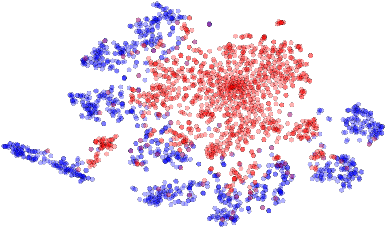
\includegraphics[width=0.45\textwidth]{./figures/adaptation_vis/pool2_mnist2inv_before.pdf}}\hfill%
  \subfigure[Adapted]{%%
    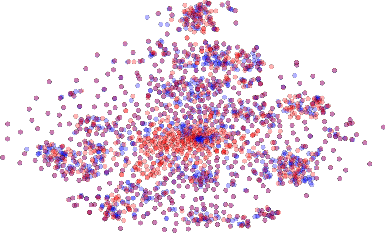
\includegraphics[width=0.45\textwidth]{./figures/adaptation_vis/pool2_mnist2inv_after.pdf}}%%
  \hspace*{\fill}%
  \end{minipage}%
  \begin{minipage}{.5\textwidth}
  \centering
  \small{{\sc Syn Numbers $ \rightarrow $ SVHN}: last hidden layer of the label predictor}
  \setcounter{subfigure}{0}
  \hspace*{\fill}%
  \subfigure[Non-adapted]{%%
    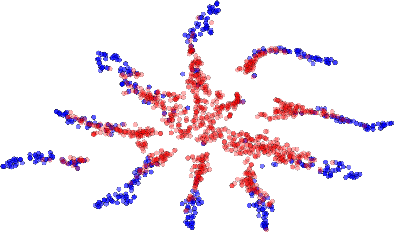
\includegraphics[width=0.45\textwidth]{./figures/adaptation_vis/before.pdf}}\hfill%
  \subfigure[Adapted]{%%
    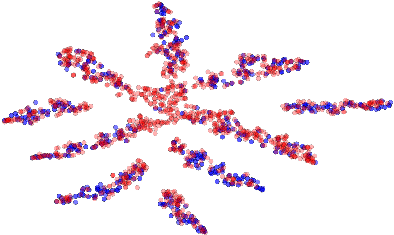
\includegraphics[width=0.45\textwidth]{./figures/adaptation_vis/after.pdf}}%%
  \hspace*{\fill}%
  \end{minipage}
  \caption{The effect of adaptation on the distribution of the extracted features (best viewed in color). The figure shows t-SNE \cite{Maaten13} visualizations of the CNN's activations {\bf (a)} in case when no adaptation was performed and {\bf (b)} in case when our adaptation procedure was incorporated into training. {\it Blue} points correspond to the source domain examples, while {\it red} ones correspond to the target domain. In all cases, the adaptation in our method makes the two distributions of features much closer.}
  \label{fig:exper_adapt_vis}
\end{figure*}

\subsection{Results}
\label{sect:exper_quant}

We now discuss the experimental settings and the results. In each case, we train on the source dataset and test on a different target domain dataset, with considerable shifts between domains (see \fig{exper_domains_examples}). The results are summarized in \tab{results} and \tab{results_office}. 

\vspace{2mm}\noindent {\bf MNIST $ \rightarrow $ MNIST-M.}
Our first experiment deals with the MNIST dataset~\cite{LeCun98} (source). In order to obtain the target domain ({\sc MNIST-M}) we blend digits from the original set over patches randomly extracted from color photos from BSDS500 \cite{Arbelaez11}. This operation is formally defined for two images $ I^{1}, I^{2} $ as $ I_{ijk}^{out} = | I_{ijk}^{1} - I_{ijk}^{2} | $, where $ i, j $ are the coordinates of a pixel and $ k $ is a channel index. In other words, an output sample is produced by taking a patch from a photo and inverting its pixels at positions corresponding to the pixels of a digit. For a human the classification task becomes only slightly harder compared to the original dataset (the digits are still clearly distinguishable) whereas for a CNN trained on MNIST this domain is quite distinct, as the background and the strokes are no longer constant. Consequently, the source-only model performs poorly. Our approach succeeded at aligning feature distributions (\fig{exper_adapt_vis}), which led to successful adaptation results (considering that the adaptation is unsupervised). At the same time, the improvement over source-only model achieved by subspace alignment (SA) \cite{Fernando13} is quite modest, thus highlighting the difficulty of the adaptation task. 

\vspace{2mm}\noindent {\bf Synthetic numbers $ \rightarrow $ SVHN.}
To address a common scenario of training on synthetic data and testing on  real data, we use Street-View House Number dataset {\sc SVHN} \cite{Netzer11} as the target domain and synthetic digits as the source. The latter ({\sc Syn ~Numbers}) consists of ~500,000 images generated by ourselves from Windows fonts by varying the text (that includes different one-, two-, and three-digit numbers), positioning, orientation, background and stroke colors, and the amount of blur. The degrees of variation were chosen manually to simulate SVHN, however the two datasets are still rather distinct, the biggest difference being the structured clutter in the background of SVHN images. 

The proposed backpropagation-based technique works well covering two thirds of the gap between training with source data only and training on target domain data with known target labels. In contrast, SA~\cite{Fernando13} does not result in any significant improvement in the classification accuracy, thus highlighting that the adaptation task is even more challenging than in the case of the MNIST experiment.

\vspace{2mm}\noindent {\bf MNIST $ \leftrightarrow $ SVHN.}
In this experiment, we further increase the gap between distributions, and test on {\sc MNIST} and {\sc SVHN}, which are significantly different in appearance. Training on SVHN even without adaptation is challenging --- classification error stays high during the first 150 epochs. In order to avoid ending up in a poor local minimum we, therefore, do not use learning rate annealing here. Obviously, the two directions ({\sc MNIST} $ \rightarrow $ {\sc SVHN} and {\sc SVHN} $ \rightarrow $ {\sc MNIST}) are not equally difficult. As {\sc SVHN} is more diverse, a model trained on SVHN is expected to be more generic and to perform reasonably on the MNIST dataset. This, indeed, turns out to be the case and is supported by the appearance of the feature distributions. We observe a quite strong separation between the domains when we feed them into the CNN trained solely on { \sc MNIST}, whereas for the {\sc SVHN}-trained network the features are much more intermixed. This difference probably explains why our method succeeded in improving the performance by adaptation in the {\sc SVHN} $ \rightarrow $ {\sc MNIST} scenario (see \tab{results}) but not in the opposite direction (SA is not able to perform adaptation in this case either). Unsupervised adaptation from MNIST to SVHN gives a failure example for our approach (we are unaware of any unsupervised DA methods capable of performing such adaptation).

\vspace{2mm}\noindent {\bf Synthetic Signs $ \rightarrow $ GTSRB.}
Overall, this setting is similar to the {\sc Syn Numbers} $ \rightarrow $ {\sc SVHN} experiment, except the distribution of the features is more complex due to the significantly larger number of classes (43 instead of 10). For the source domain we obtained~100,000 synthetic images (which we call {\sc Syn~Signs}) simulating various photoshooting conditions. Once again, our method achieves a sensible increase in performance once again proving its suitability for the synthetic-to-real data adaptation.

\begin{figure}
  \centering
  \setlength\figureheight{2.7cm}
  \setlength\figurewidth{6.8cm}
  % This file was created by matlab2tikz v0.5.0 running on MATLAB 8.3.
%Copyright (c) 2008--2014, Nico Schlömer <nico.schloemer@gmail.com>
%All rights reserved.
%Minimal pgfplots version: 1.3
%
%The latest updates can be retrieved from
%  http://www.mathworks.com/matlabcentral/fileexchange/22022-matlab2tikz
%where you can also make suggestions and rate matlab2tikz.
%
\begin{tikzpicture}[font=\scriptsize]

\begin{axis}[%
width=0.95092\figurewidth,
height=\figureheight,
at={(0\figurewidth,0\figureheight)},
scale only axis,
xmin=10000,
xmax=50000,
xlabel={Batches seen},
ymin=0,
ymax=1,
ylabel={Validation error},
axis x line*=bottom,
axis y line*=left,
legend style={at={($ (1,1) + (-0.1cm,-0.1cm) $)},anchor=north east,align=left,legend cell align=left,draw=black},
xmajorgrids,
ymajorgrids,
grid style={dashed}
]
\addplot [color=blue,solid,line width=1.0pt]
  table[row sep=crcr]{%
10500	0.199757996632997\\
11000	0.19162984006734\\
11500	0.190788089225589\\
12000	0.192918771043771\\
12500	0.196390993265993\\
13000	0.185527146464646\\
13500	0.190472432659933\\
14000	0.185606060606061\\
14500	0.183422769360269\\
15000	0.189051978114478\\
15500	0.191524621212121\\
16000	0.186079545454545\\
16500	0.179424452861953\\
17000	0.187684132996633\\
17500	0.187868265993266\\
18000	0.180923821548822\\
18500	0.187315867003367\\
19000	0.178661616161616\\
19500	0.18102904040404\\
20000	0.180555555555556\\
20500	0.176662457912458\\
21000	0.183791035353535\\
21500	0.179214015151515\\
22000	0.178898358585859\\
22500	0.178898358585859\\
23000	0.174479166666667\\
23500	0.174742213804714\\
24000	0.171059553872054\\
24500	0.177951388888889\\
25000	0.174794823232323\\
25500	0.174084595959596\\
26000	0.174636994949495\\
26500	0.169034090909091\\
27000	0.171191077441077\\
27500	0.170875420875421\\
28000	0.171506734006734\\
28500	0.170217803030303\\
29000	0.169244528619529\\
29500	0.169875841750842\\
30000	0.168744739057239\\
30500	0.17048085016835\\
31000	0.169454966329966\\
31500	0.167771464646465\\
32000	0.168849957912458\\
32500	0.168323863636364\\
33000	0.168718434343434\\
33500	0.165667087542088\\
34000	0.167376893939394\\
34500	0.169007786195286\\
35000	0.167140151515152\\
35500	0.165667087542088\\
36000	0.167850378787879\\
36500	0.169823232323232\\
37000	0.170691287878788\\
37500	0.16640361952862\\
38000	0.167981902356902\\
38500	0.169875841750842\\
39000	0.166771885521886\\
39500	0.169376052188552\\
40000	0.168087121212121\\
40500	0.165509259259259\\
41000	0.167718855218855\\
41500	0.168060816498317\\
42000	0.166035353535354\\
42500	0.166692971380471\\
43000	0.166429924242424\\
43500	0.167034932659933\\
44000	0.170349326599327\\
44500	0.169744318181818\\
45000	0.168218644781145\\
45500	0.166429924242424\\
46000	0.166324705387205\\
46500	0.168771043771044\\
47000	0.168034511784512\\
47500	0.168718434343434\\
48000	0.171059553872054\\
48500	0.170638678451178\\
49000	0.16819234006734\\
49500	0.168981481481481\\
50000	0.167902988215488\\
};
\addlegendentry{Real data only};

\addplot [color=cyan,solid,line width=1.0pt]
  table[row sep=crcr]{%
10500	0.9625\\
11000	0.79765625\\
11500	0.715625\\
12000	0.6140625\\
12500	0.52109375\\
13000	0.459375\\
13500	0.4484375\\
14000	0.421875\\
14500	0.39453125\\
15000	0.4109375\\
15500	0.34296875\\
16000	0.36875\\
16500	0.3359375\\
17000	0.36171875\\
17500	0.3171875\\
18000	0.3484375\\
18500	0.32421875\\
19000	0.315625\\
19500	0.346875\\
20000	0.31875\\
20500	0.35390625\\
21000	0.3265625\\
21500	0.33359375\\
22000	0.3171875\\
22500	0.28515625\\
23000	0.30546875\\
23500	0.309375\\
24000	0.2796875\\
24500	0.30859375\\
25000	0.30703125\\
25500	0.3078125\\
26000	0.28671875\\
26500	0.2875\\
27000	0.31484375\\
27500	0.2859375\\
28000	0.29375\\
28500	0.31328125\\
29000	0.3078125\\
29500	0.2859375\\
30000	0.2890625\\
30500	0.284375\\
31000	0.2953125\\
31500	0.26953125\\
32000	0.29921875\\
32500	0.30078125\\
33000	0.2640625\\
33500	0.309375\\
34000	0.2734375\\
34500	0.290625\\
35000	0.26796875\\
35500	0.3015625\\
36000	0.26796875\\
36500	0.2921875\\
37000	0.265625\\
37500	0.2765625\\
38000	0.2859375\\
38500	0.32109375\\
39000	0.28046875\\
39500	0.275\\
40000	0.24921875\\
40500	0.29140625\\
41000	0.26640625\\
41500	0.265625\\
42000	0.259375\\
42500	0.2765625\\
43000	0.26796875\\
43500	0.2765625\\
44000	0.27265625\\
44500	0.25546875\\
45000	0.26484375\\
45500	0.271875\\
46000	0.2703125\\
46500	0.26171875\\
47000	0.246875\\
47500	0.25078125\\
48000	0.29609375\\
48500	0.2640625\\
49000	0.26875\\
49500	0.26015625\\
50000	0.2578125\\
};
\addlegendentry{Synthetic data only};

\addplot [color=red,solid,line width=1.0pt]
  table[row sep=crcr]{%
10500	0.943892045454545\\
11000	0.943892045454545\\
11500	0.943892045454545\\
12000	0.943892045454545\\
12500	0.848300715488216\\
13000	0.658722643097643\\
13500	0.590593434343434\\
14000	0.475484006734007\\
14500	0.313946759259259\\
15000	0.235690235690236\\
15500	0.17879313973064\\
16000	0.152383207070707\\
16500	0.12912984006734\\
17000	0.114478114478114\\
17500	0.116214225589226\\
18000	0.1015625\\
18500	0.10066813973064\\
19000	0.101983375420875\\
19500	0.0914351851851852\\
20000	0.0895675505050505\\
20500	0.0894360269360269\\
21000	0.0827283249158249\\
21500	0.0798611111111111\\
22000	0.0859638047138047\\
22500	0.0799137205387205\\
23000	0.0778619528619529\\
23500	0.0737584175084175\\
24000	0.0742582070707071\\
24500	0.0776778198653199\\
25000	0.0771517255892256\\
25500	0.0725747053872054\\
26000	0.0739425505050505\\
26500	0.0734953703703704\\
27000	0.0730744949494949\\
27500	0.0688920454545455\\
28000	0.0702072811447811\\
28500	0.072337962962963\\
29000	0.0670244107744108\\
29500	0.0733638468013468\\
30000	0.0667613636363636\\
30500	0.0692340067340067\\
31000	0.0652093855218855\\
31500	0.0664720117845118\\
32000	0.0655776515151515\\
32500	0.0671296296296296\\
33000	0.0656039562289562\\
33500	0.0646043771043771\\
34000	0.0668665824915825\\
34500	0.0638678451178451\\
35000	0.065077861952862\\
35500	0.0649989478114478\\
36000	0.0672348484848485\\
36500	0.0668665824915825\\
37000	0.0626052188552189\\
37500	0.0652093855218855\\
38000	0.0626315235690236\\
38500	0.0627893518518518\\
39000	0.0613162878787879\\
39500	0.063236531986532\\
40000	0.0629208754208754\\
40500	0.0639467592592593\\
41000	0.0612899831649832\\
41500	0.0653409090909091\\
42000	0.0608691077441077\\
42500	0.0613425925925926\\
43000	0.0630260942760943\\
43500	0.060106271043771\\
44000	0.0638678451178451\\
44500	0.0602377946127946\\
45000	0.0577388468013468\\
45500	0.062684132996633\\
46000	0.0608164983164983\\
46500	0.0603167087542088\\
47000	0.0577651515151515\\
47500	0.0583175505050505\\
48000	0.0591329966329966\\
48500	0.0607112794612795\\
49000	0.0585805976430976\\
49500	0.0583175505050505\\
50000	0.0590540824915825\\
};
\addlegendentry{Both};

\end{axis}
\end{tikzpicture}%
  \caption{Semi-supervised domain adaptation for the traffic signs. As labeled target domain data are shown to the method, it achieves significantly lower error than the model trained on target domain data only or on source domain data only. \vspace{-4mm}}
  \label{fig:exper_semi_test}
\end{figure}

As an additional experiment, we also evaluate the proposed algorithm for semi-supervised domain adaptation, i.e.\ when one is additionally provided with a small amount of labeled target data. For that purpose we split {\sc GTSRB} into the train set (1280 random samples with labels) and the validation set (the rest of the dataset). The validation part is used solely for the evaluation and does not participate in the adaptation. The training procedure changes slightly as the label predictor is now exposed to the target data. \fig{exper_semi_test} shows the change of the validation error throughout the training. While the graph clearly suggests that our method can be used in the semi-supervised setting, thorough verification of semi-supervised setting is left for future work.


\vspace{2mm}\noindent {\bf Office dataset.} 
We finally evaluate our method on {\sc Office} dataset, which is a collection of three distinct domains: {\sc Amazon}, {\sc DSLR}, and {\sc Webcam}. Unlike previously discussed datasets, {\sc Office} is rather small-scale with only 2817 labeled images spread across 31 different categories in the largest domain. The amount of available data is crucial for a successful training of a deep model, hence we opted for the fine-tuning of the CNN pre-trained on the ImageNet \cite{Jia14} as it is done in some recent DA works \cite{Donahue14,Tzeng14,Hoffman14}. We make our approach more comparable with \cite{Tzeng14} by using exactly the same network architecture replacing domain mean-based regularization with the domain classifier.

Following most previous works, we evaluate our method using 5 random splits for each of the 3 transfer tasks commonly used for evaluation. Our training protocol is close to \cite{Tzeng14,Saenko10,Gong12} as we use the same number of labeled source-domain images per category. Unlike those works and similarly to e.g.\ DLID~\cite{Chopra13} we use the whole unlabeled target domain (as the premise of our method is the abundance of unlabeled data in the target domain). Under this transductive setting, our method is able to improve previously-reported state-of-the-art accuracy for unsupervised adaptation very considerably (\tab{results_office}), especially in the most challenging {\sc Amazon} $ \rightarrow $ {\sc Webcam} scenario (the two domains with the largest domain shift).

\section{Conclusion}
\label{conclusions}
The supervised paradigm for training machine reading and comprehension models
provides a promising avenue for making progress on the path to building full
natural language understanding systems. We have demonstrated a methodology for
obtaining a large number of document-query-answer triples and shown that
recurrent and attention based neural networks provide an effective modelling
framework for this task.
Our analysis indicates that the Attentive and Impatient Readers are able to
propagate and integrate semantic information over long distances. In particular
we believe that the incorporation of an attention mechanism is the key
contributor to these results.


The attention mechanism
that we have employed is just one instantiation of a very general idea which
can be further exploited. However, the incorporation of world knowledge and
multi-document queries will also require the development of attention and
embedding mechanisms whose complexity to query does not scale linearly with the
data set size.
There are still many queries requiring complex inference and long range reference resolution that our models are not yet able to answer. As such our data provides a scalable challenge that should support NLP research into the future. Further, significantly bigger training data sets can be acquired using the techniques we have described, undoubtedly allowing us to train more expressive and accurate models.


\subsubsection*{Acknowledgments}
The authors would like to thank David Grangier, Tomas Mikolov, Leon Bottou, Ronan Collobert and Laurens van der Maaten for their insightful comments. 
We also would like to thank Alexander M. Rush for his help in preparing the data set for the summarization task and Sam Gross for providing the image features. 

\bibliography{iclr2016_conference}
\bibliographystyle{iclr2016_conference}
\newpage
\section{Supplementary Material}


\subsection{Experiments}


\subsubsection{Qualitative Comparison}
\begin{figure}[h!]
\tiny{
\begin{verbatim}


CONTEXT:      a chinese government official on sunday dismissed reports that the government was delaying the issuing
              of third generation -lrb- #g -rrb- mobile phone licenses in order to give a developing <unk> system an
              advantage
GROUND TRUTH: foreign phone operators to get equal access to china 's #g market
XENT:         china dismisses report of #g mobile phone phone
DAD:          china denies <unk> <unk> mobile phone licenses
E2E:          china 's mobile phone licenses delayed
MIXER:        china official dismisses reports of #g mobile licenses

CONTEXT:      greece risks bankruptcy if it does not take radical extra measures to fix its finances , prime minister
              george papandreou warned on tuesday , saying the country was in a `` wartime situation
GROUND TRUTH: greece risks bankruptcy without radical action
XENT:         greece warns <unk> measures to <unk> finances
DAD:          greece says no measures to <unk> <unk>
E2E:          greece threatens to <unk> measures to <unk> finances
MIXER:        greece does not take radical measures to <unk> deficit

CONTEXT:      the indonesian police were close to identify the body parts resulted from the deadly explosion in front
              of the australian embassy by the dna test , police chief general <unk> <unk> said on wednesday
GROUND TRUTH: indonesian police close to <unk> australian embassy bomber
XENT:         indonesian police close to <unk>
DAD:          indonesian police close to <unk>
E2E:          indonesian police close to monitor deadly australia
MIXER:        indonesian police close to <unk> parts of australian embassy

CONTEXT:      hundreds of catholic and protestant youths attacked security forces with <unk> bombs in a flashpoint
              area of north belfast late thursday as violence erupted for the second night in a row , police said
GROUND TRUTH: second night of violence erupts in north belfast
XENT:         urgent hundreds of catholic and <unk> <unk> in <unk>
DAD:          hundreds of belfast <unk> <unk> in n. belfast
E2E:          hundreds of catholic protestant , <unk> clash with <unk>
MIXER:        hundreds of catholic <unk> attacked in north belfast

CONTEXT:      uganda 's lord 's resistance army -lrb- lra -rrb- rebel leader joseph <unk> is planning to join his
              commanders in the ceasefire area ahead of talks with the government , ugandan army has said
GROUND TRUTH: rebel leader to move to ceasefire area         
XENT:         uganda 's <unk> rebel leader to join ceasefire
DAD:          ugandan rebel leader to join ceasefire talks
E2E:          ugandan rebels <unk> rebel leader
MIXER:        ugandan rebels to join ceasefire in <unk>

CONTEXT:      a russian veterinary official reported a fourth outbreak of dead domestic poultry in a suburban
              moscow district sunday as experts tightened <unk> following confirmation of the presence of the 
              deadly h#n# bird flu strain
GROUND TRUTH: tests confirm h#n# bird flu strain in # <unk> moscow <unk>
XENT:         russian official reports fourth flu in <unk>
DAD:          bird flu outbreak in central china
E2E:          russian official official says outbreak outbreak outbreak in <unk>
MIXER:        russian official reports fourth bird flu

CONTEXT:      a jewish human rights group announced monday that it will offer <unk> a dlrs ##,### reward for 
              information that helps them track down those suspected of participating in nazi atrocities during 
              world war ii
GROUND TRUTH: jewish human rights group offers reward for information on nazi suspects in lithuania
XENT:         jewish rights group announces <unk> to reward for war during world war
DAD:          rights group announces <unk> dlrs dlrs dlrs reward
E2E:          jewish rights group offers reward for <unk>
MIXER:        jewish human rights group to offer reward for <unk>

CONTEXT:      a senior u.s. envoy reassured australia 's opposition labor party on saturday that no decision 
              had been made to take military action against iraq and so no military assistance had been sought 
              from australia
GROUND TRUTH: u.s. envoy meets opposition labor party to discuss iraq
XENT:         australian opposition party makes progress on military action against iraq
DAD:          australian opposition party says no military action against iraq
E2E:          us envoy says no decision to take australia 's labor
MIXER:        u.s. envoy says no decision to military action against iraq

CONTEXT:      republican u.s. presidential candidate rudy giuliani met privately wednesday with iraqi president 
              jalal talabani and indicated that he would keep a u.s. presence in iraq for as long as necessary , 
              campaign aides said
GROUND TRUTH: giuliani meets with iraqi president , discusses war
XENT:         <unk> meets with president of iraqi president
DAD:          republican presidential candidate meets iraqi president
E2E:          u.s. president meets with iraqi president
MIXER:        u.s. presidential candidate giuliani meets with iraqi president
\end{verbatim}
}
\caption{Examples of greedy generations after conditioning on sentences from the test summarization dataset. The "$<$unk$>$" token is produced by our tokenizer and it replaces rare words.} 
\label{fig:generation}
\end{figure}


\subsubsection{Hyperparameters}
\begin{table}[!h]
\caption{Best scheduling parameters found by hyper-parameter search of MIXER.}
\begin{tabular}{l || l | l | l}
      \multicolumn{1}{c||}{\emph{TASK} }  & 
      \multicolumn{1}{c|}{$N^{\mbox{\small XENT}}$} & 
      \multicolumn{1}{c|}{$N^{\mbox{\small XE+R}}$} & \multicolumn{1}{c}{$\Delta$} \\
      \hline
      \hline
      {\em summarization} & 20 & 5 & 2  \\
      \hline
      {\em machine translation} & 25 & 5 & 3 \\
      \hline
      {\em image captioning} & 20 & 5 & 2  \\
    \end{tabular}
\label{tab:scheduling}
\end{table}

\subsubsection{Relative Gains}


\begin{figure}[!h]
\begin{center}
 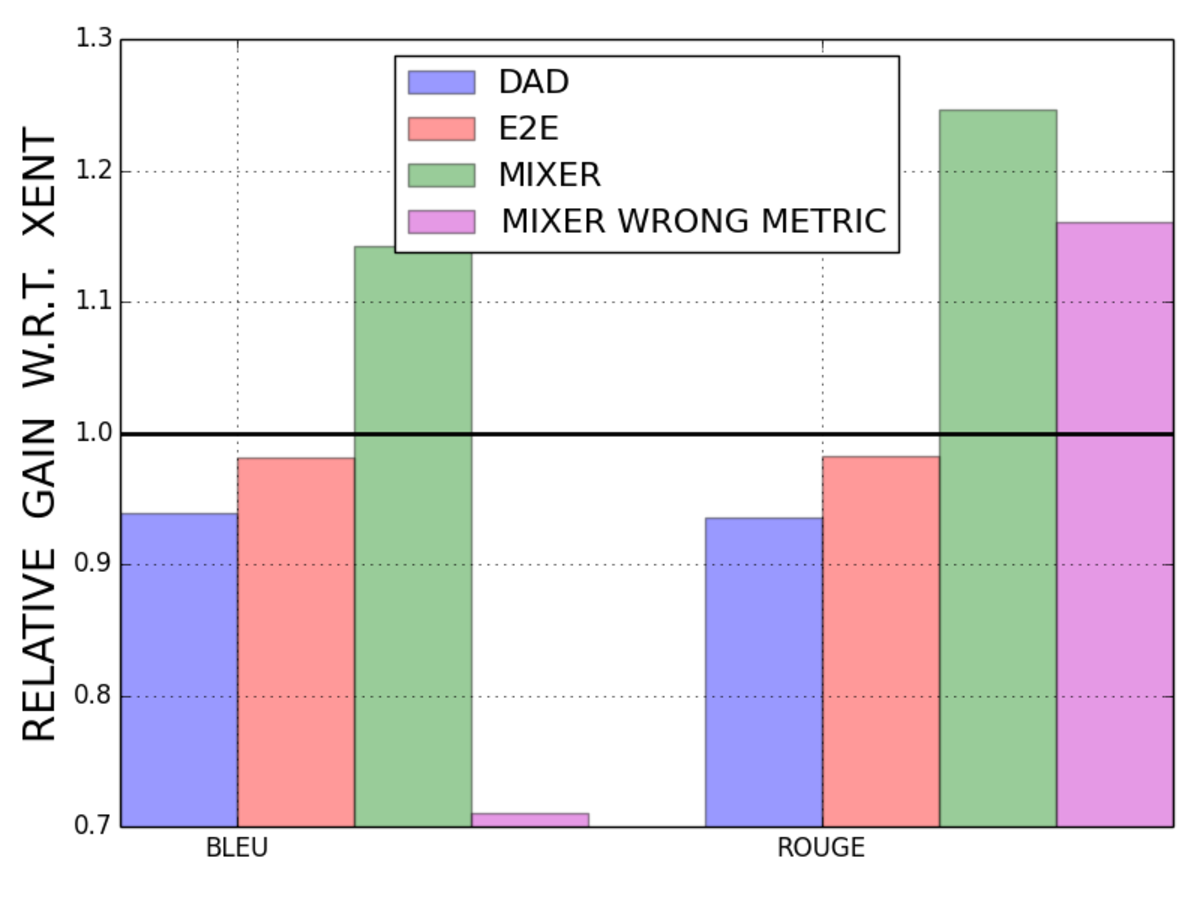
\includegraphics[width=0.6\linewidth]{summarization_bleu_rouge.pdf}
 \end{center}
\caption{Relative gains on summarization with respect to the XENT baseline. Left: relative BLEU score. Right: relative ROUGE-2.
The models are: DAD, E2E, MIXER trained for the objective used at test time (method proposed in this paper), and MIXER trained with a different metric.
When evaluating for BLEU, the last column on the left reports the evaluation of MIXER trained using ROUGE-2.
When evaluating for ROUGE-2, the last column on the right reports the evaluation of MIXER trained using BLEU.}
\label{fig:summarization_bleu_rouge}
\end{figure}



\vspace{0.3in}
\begin{figure}[!h]
  \centering
  \begin{minipage}{0.05\linewidth}
  	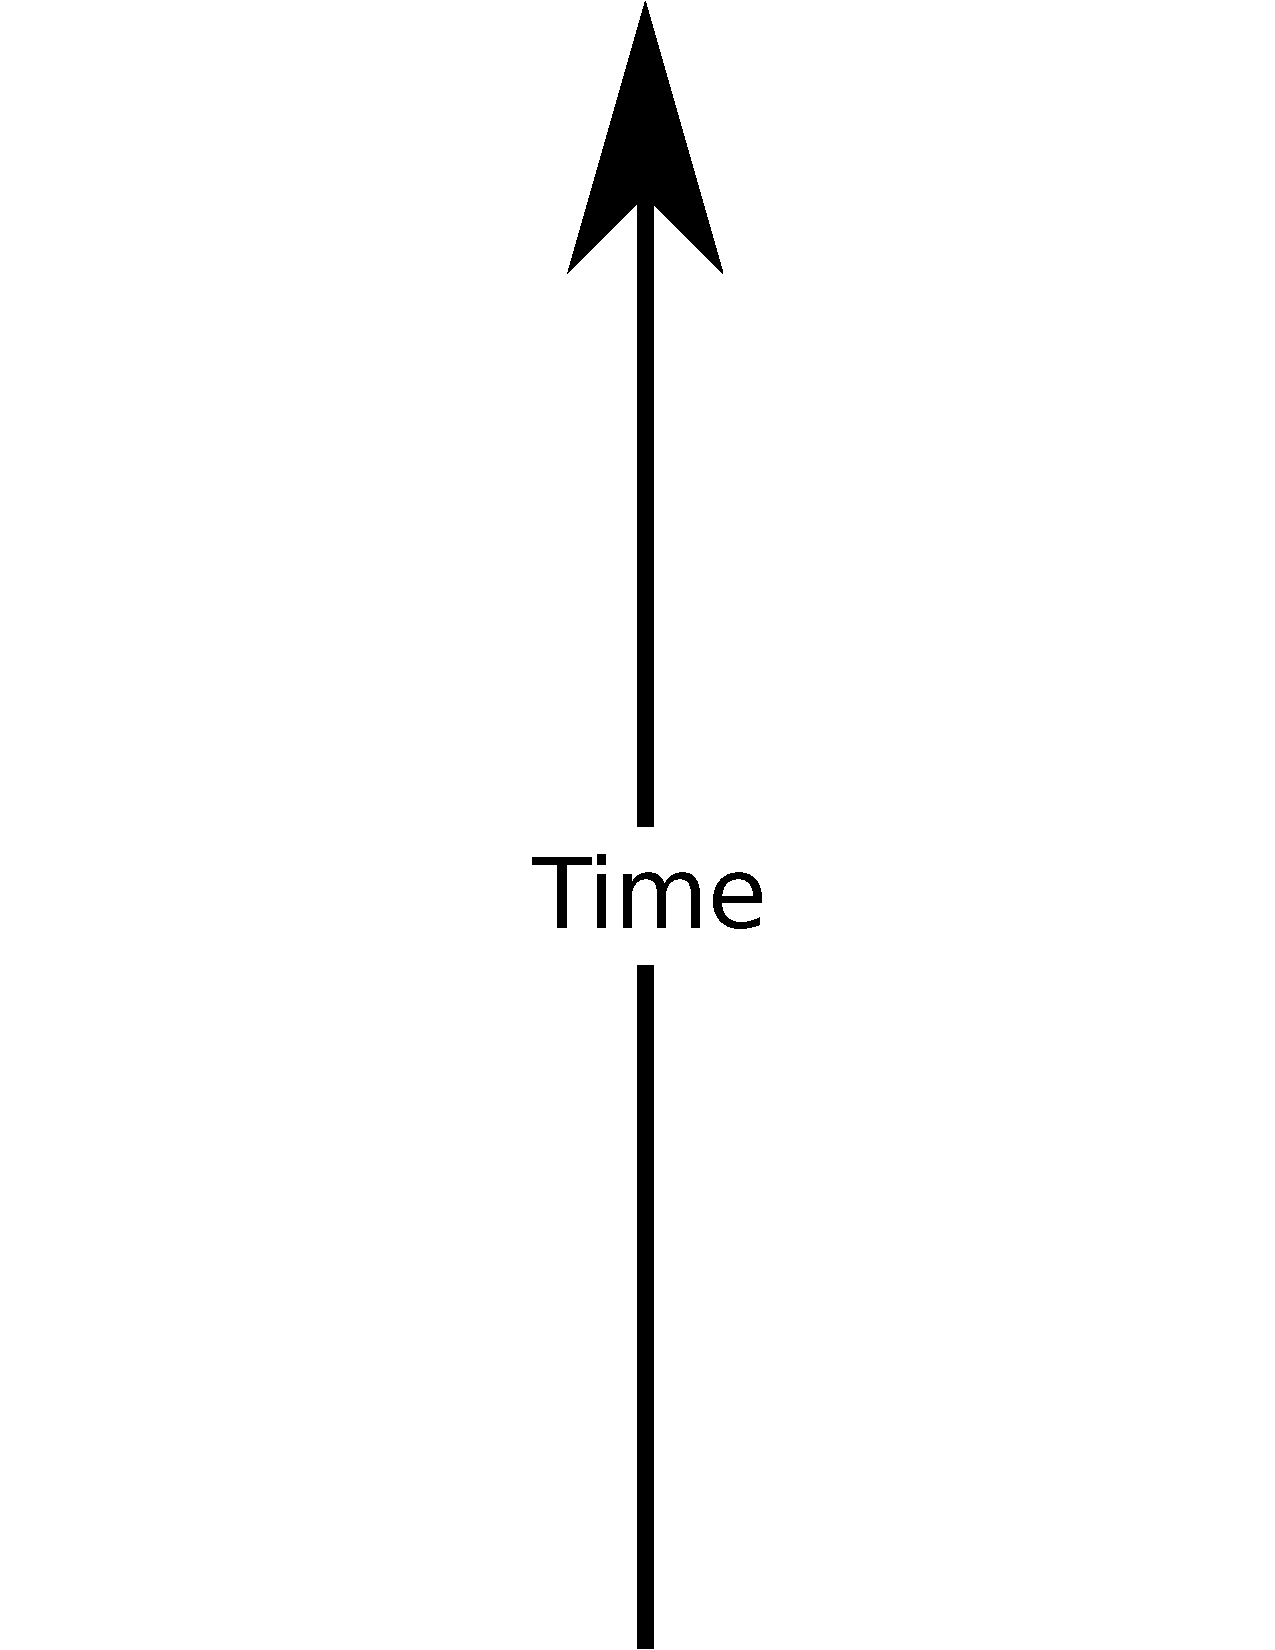
\includegraphics[width=2.5\linewidth]{time.pdf}\\
  \end{minipage}
  \begin{minipage}{0.46\linewidth}
  	\centering
    \scalebox{0.75}{
    \tiny
    \begingroup\makeatletter\def\f@size{1}\check@mathfonts
    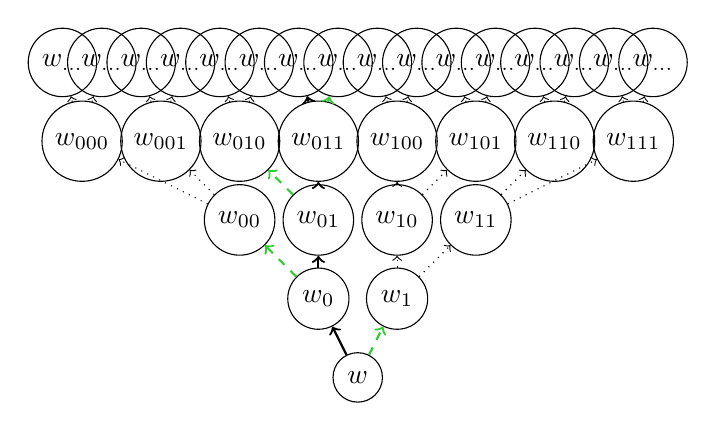
\begin{tikzpicture}
      \node [draw, circle] (w) at (0,0) {$w$};
      \node [draw, circle] (w0) at (-0.5,1) {$w_0$};
      \node [draw, circle] (w1) at (0.5,1) {$w_1$};
      \node [draw, circle] (w00) at (-1.5,2) {$w_{00}$};
      \node [draw, circle] (w01) at (-0.5,2) {$w_{01}$};
      \node [draw, circle] (w10) at (0.5,2) {$w_{10}$};
      \node [draw, circle] (w11) at (1.5,2) {$w_{11}$};
      \node [draw, circle] (w000) at (-3.5,3) {$w_{000}$};
      \node [draw, circle] (w001) at (-2.5,3) {$w_{001}$};
      \node [draw, circle] (w010) at (-1.5,3) {$w_{010}$};
      \node [draw, circle] (w011) at (-0.5,3) {$w_{011}$};
      \node [draw, circle] (w100) at (0.5,3) {$w_{100}$};
      \node [draw, circle] (w101) at (1.5,3) {$w_{101}$};
      \node [draw, circle] (w110) at (2.5,3) {$w_{110}$};
      \node [draw, circle] (w111) at (3.5,3) {$w_{111}$};
      \node [draw, circle] (w0000) at (-3.75,4) {$w_{\dots}$};
      \node [draw, circle] (w0001) at (-3.25,4) {$w_{\dots}$};
      \node [draw, circle] (w0010) at (-2.75,4) {$w_{\dots}$};
      \node [draw, circle] (w0011) at (-2.25,4) {$w_{\dots}$};
      \node [draw, circle] (w0100) at (-1.75,4) {$w_{\dots}$};
      \node [draw, circle] (w0101) at (-1.25,4) {$w_{\dots}$};
      \node [draw, circle] (w0110) at (-0.75,4) {$w_{\dots}$};
      \node [draw, circle] (w0111) at (-0.25,4) {$w_{\dots}$};
      \node [draw, circle] (w1000) at (0.25,4) {$w_{\dots}$};
      \node [draw, circle] (w1001) at (0.75,4) {$w_{\dots}$};
      \node [draw, circle] (w1010) at (1.25,4) {$w_{\dots}$};
      \node [draw, circle] (w1011) at (1.75,4) {$w_{\dots}$};
      \node [draw, circle] (w1100) at (2.25,4) {$w_{\dots}$};
      \node [draw, circle] (w1101) at (2.75,4) {$w_{\dots}$};
      \node [draw, circle] (w1110) at (3.25,4) {$w_{\dots}$};
      \node [draw, circle] (w1111) at (3.75,4) {$w_{\dots}$};
      \draw [thick] [->] (w) to (w0);
      \draw [thick] [dashed] [green] [->] (w) to (w1);
      \draw [thick] [dashed] [green] [->] (w0) to (w00);
      \draw [thick] [->] (w0) to (w01);
      \draw [dotted] [->] (w1) to (w10);
      \draw [dotted] [->] (w1) to (w11);
      \draw [dotted] [->] (w00) to (w000);
      \draw [dotted] [->] (w00) to (w001);
      \draw [thick] [dashed] [green] [->] (w01) to (w010);
      \draw [thick] [->] (w01) to (w011);
      \draw [dotted] [->] (w10) to (w100);
      \draw [dotted] [->] (w10) to (w101);
      \draw [dotted] [->] (w11) to (w110);
      \draw [dotted] [->] (w11) to (w111);
      \draw [dotted] [->] (w000) to (w0000);
      \draw [dotted] [->] (w000) to (w0001);
      \draw [dotted] [->] (w001) to (w0010);
      \draw [dotted] [->] (w001) to (w0011);
      \draw [dotted] [->] (w010) to (w0100);
      \draw [dotted] [->] (w010) to (w0101);
      \draw [thick] [->] (w011) to (w0110);
      \draw [thick] [dashed] [green] [->] (w011) to (w0111);
      \draw [dotted] [->] (w100) to (w1000);
      \draw [dotted] [->] (w100) to (w1001);
      \draw [dotted] [->] (w101) to (w1010);
      \draw [dotted] [->] (w101) to (w1011);
      \draw [dotted] [->] (w110) to (w1100);
      \draw [dotted] [->] (w110) to (w1101);
      \draw [dotted] [->] (w111) to (w1110);
      \draw [dotted] [->] (w111) to (w1111);
      \end{tikzpicture}
      \endgroup
    }\\
    Training with exposure bias
  \end{minipage}
  \begin{minipage}{0.46\linewidth}
  	\centering
    \scalebox{0.75}{
    \tiny
    \begingroup\makeatletter\def\f@size{1}\check@mathfonts
    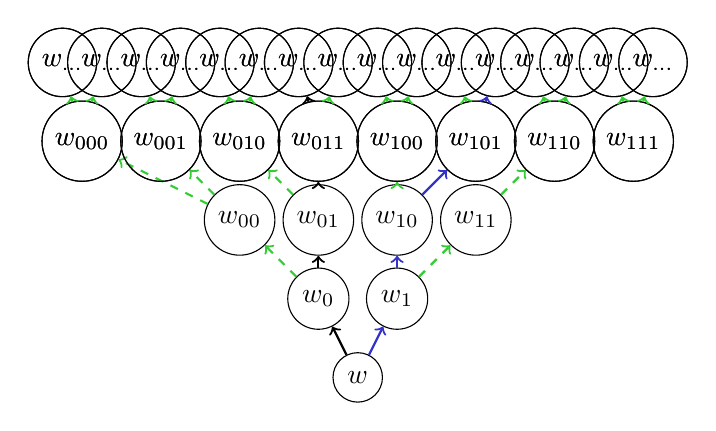
\begin{tikzpicture}
      \node [draw, circle] (w) at (0,0) {$w$};
      \node [draw, circle] (w0) at (-0.5,1) {$w_0$};
      \node [draw, circle] (w1) at (0.5,1) {$w_1$};
      \node [draw, circle] (w00) at (-1.5,2) {$w_{00}$};
      \node [draw, circle] (w01) at (-0.5,2) {$w_{01}$};
      \node [draw, circle] (w10) at (0.5,2) {$w_{10}$};
      \node [draw, circle] (w11) at (1.5,2) {$w_{11}$};
      \node [draw, circle] (w000) at (-3.5,3) {$w_{000}$};
      \node [draw, circle] (w001) at (-2.5,3) {$w_{001}$};
      \node [draw, circle] (w010) at (-1.5,3) {$w_{010}$};
      \node [draw, circle] (w011) at (-0.5,3) {$w_{011}$};
      \node [draw, circle] (w100) at (0.5,3) {$w_{100}$};
      \node [draw, circle] (w101) at (1.5,3) {$w_{101}$};
      \node [draw, circle] (w110) at (2.5,3) {$w_{110}$};
      \node [draw, circle] (w111) at (3.5,3) {$w_{111}$};
      \node [draw, circle] (w0000) at (-3.75,4) {$w_{\dots}$};
      \node [draw, circle] (w0001) at (-3.25,4) {$w_{\dots}$};
      \node [draw, circle] (w0010) at (-2.75,4) {$w_{\dots}$};
      \node [draw, circle] (w0011) at (-2.25,4) {$w_{\dots}$};
      \node [draw, circle] (w0100) at (-1.75,4) {$w_{\dots}$};
      \node [draw, circle] (w0101) at (-1.25,4) {$w_{\dots}$};
      \node [draw, circle] (w0110) at (-0.75,4) {$w_{\dots}$};
      \node [draw, circle] (w0111) at (-0.25,4) {$w_{\dots}$};
      \node [draw, circle] (w1000) at (0.25,4) {$w_{\dots}$};
      \node [draw, circle] (w1001) at (0.75,4) {$w_{\dots}$};
      \node [draw, circle] (w1010) at (1.25,4) {$w_{\dots}$};
      \node [draw, circle] (w1011) at (1.75,4) {$w_{\dots}$};
      \node [draw, circle] (w1100) at (2.25,4) {$w_{\dots}$};
      \node [draw, circle] (w1101) at (2.75,4) {$w_{\dots}$};
      \node [draw, circle] (w1110) at (3.25,4) {$w_{\dots}$};
      \node [draw, circle] (w1111) at (3.75,4) {$w_{\dots}$};

      \draw [thick] [->] (w) to (w0);
      \draw [thick] [blue] [->] (w) to (w1);
      \draw [thick] [dashed] [green] [->] (w0) to (w00);
      \draw [thick] [->] (w0) to (w01);
      \draw [thick] [blue] [->] (w1) to (w10);
      \draw [thick] [dashed] [green] [->] (w1) to (w11);
      \draw [thick] [dashed] [green] [->] (w00) to (w000);
      \draw [thick] [dashed] [green] [->] (w00) to (w001);
      \draw [thick] [dashed] [green] [->] (w01) to (w010);
      \draw [thick] [->] (w01) to (w011);
      \draw [thick] [dashed] [green] [->] (w10) to (w100);
      \draw [thick] [blue] [->] (w10) to (w101);
      \draw [thick] [dashed] [green] [->] (w11) to (w110);
      \node [draw, circle] (w000) at (-3.5,3) {$w_{000}$};
      \node [draw, circle] (w001) at (-2.5,3) {$w_{001}$};
      \node [draw, circle] (w010) at (-1.5,3) {$w_{010}$};
      \node [draw, circle] (w011) at (-0.5,3) {$w_{011}$};
      \node [draw, circle] (w100) at (0.5,3) {$w_{100}$};
      \node [draw, circle] (w101) at (1.5,3) {$w_{101}$};
      \node [draw, circle] (w110) at (2.5,3) {$w_{110}$};
      \node [draw, circle] (w111) at (3.5,3) {$w_{111}$};
      \node [draw, circle] (w0000) at (-3.75,4) {$w_{\dots}$};
      \node [draw, circle] (w0001) at (-3.25,4) {$w_{\dots}$};
      \node [draw, circle] (w0010) at (-2.75,4) {$w_{\dots}$};
      \node [draw, circle] (w0011) at (-2.25,4) {$w_{\dots}$};
      \node [draw, circle] (w0100) at (-1.75,4) {$w_{\dots}$};
      \node [draw, circle] (w0101) at (-1.25,4) {$w_{\dots}$};
      \node [draw, circle] (w0110) at (-0.75,4) {$w_{\dots}$};
      \node [draw, circle] (w0111) at (-0.25,4) {$w_{\dots}$};
      \node [draw, circle] (w1000) at (0.25,4) {$w_{\dots}$};
      \node [draw, circle] (w1001) at (0.75,4) {$w_{\dots}$};
      \node [draw, circle] (w1010) at (1.25,4) {$w_{\dots}$};
      \node [draw, circle] (w1011) at (1.75,4) {$w_{\dots}$};
      \node [draw, circle] (w1100) at (2.25,4) {$w_{\dots}$};
      \node [draw, circle] (w1101) at (2.75,4) {$w_{\dots}$};
      \node [draw, circle] (w1110) at (3.25,4) {$w_{\dots}$};
      \node [draw, circle] (w1111) at (3.75,4) {$w_{\dots}$};
      \draw [thick] [dashed] [green] [->] (w000) to (w0000);
      \draw [thick] [dashed] [green] [->] (w000) to (w0001);
      \draw [thick] [dashed] [green] [->] (w001) to (w0010);
      \draw [thick] [dashed] [green] [->] (w001) to (w0011);
      \draw [thick] [dashed] [green] [->] (w010) to (w0100);
      \draw [thick] [dashed] [green] [->] (w010) to (w0101);
      \draw [thick] [->] (w011) to (w0110);
      \draw [thick] [dashed] [green] [->] (w011) to (w0111);
      \draw [thick] [dashed] [green] [->] (w100) to (w1000);
      \draw [thick] [dashed] [green] [->] (w100) to (w1001);
      \draw [thick] [dashed] [green] [->] (w101) to (w1010);
      \draw [thick] [blue] [->] (w101) to (w1011);
      \draw [thick] [dashed] [green] [->] (w110) to (w1100);
      \draw [thick] [dashed] [green] [->] (w110) to (w1101);
      \draw [thick] [dashed] [green] [->] (w111) to (w1110);
      \draw [thick] [dashed] [green] [->] (w111) to (w1111);
      \end{tikzpicture}
      \endgroup
    }
	Training in expectation (Reinforce)
  \end{minipage}
  \caption{Search space for the toy case of a binary vocabulary and sequences of length 4.  
    The trees represent all the $2^4$ possible sequences.
  The solid black line is the ground truth sequence. 
  \textbf{(Left)} Greedy training such as XENT optimizes only the probability 
  of the next word. The model may consider choices indicated by the green arrows, but it starts off from words taken from the ground truth sequence. The model experiences exposure bias, since it sees only words branching off the ground truth path;
  \textbf{(Right)} REINFORCE and MIXER optimize over all possible sequences, using the predictions made by the model itself.  
  In practice, the model samples only a single path indicated by the blue solid line. The model does not suffer from exposure bias; the model is trained as it is tested.}
  \label{fig:plan}
\end{figure}

  


    


\subsection{The Attentive Encoder}
\label{sup-material:encoder}
Here we explain in detail how we generate the conditioning vector $\bc_t$ 
for our RNN using the source sentence and the current hidden state $\bh_t$. 
Let us denote by $\bs$ the source sentence which is composed of a sequence 
of $M$ words $\bs = [w_1, \ldots, w_M]$. 
With a slight overload of notation let $w_i$ also denote the $d$ dimensional 
learnable embedding of the $i$-th word ($w_i \in \setr^d$). In addition the 
position $i$ of the word $w_i$ is also associated with a learnable embedding $l_i$ 
of size $d$ ($l_i \in \setr^d$). Then the full embedding for 
the $i$-th word in the input sentence is given by $a_i = w_i + l_i$. 
In order for the embeddings to capture local context, we associate an 
aggregate embedding $z_i$ to each word in the source sentence. 
In particular for a word in the $i$-th position, its aggregate embedding 
$z_i$ is computed by taking a window of $q$ consecutive words centered 
at position $i$ and averaging the embeddings of all the words in this window. More precisely, the aggregate embedding $z_i$ is given by: 
\begin{equation}
z_i = \frac{1}{q} \sum_{h = -q/2}^{q/2} a_{i + h}. 
\end{equation}
In our experiments the width $q$ was set to $5$. 
In order to account for the words at the two boundaries of the input 
sentence we first pad the sequence on both sides with dummy words before 
computing the aggregate vectors $z_i$s. Given these aggregate vectors of words, we compute 
the context vector $c_t$ (the final output of the encoder) as: 
\begin{equation}
c_t = \sum_{j=1}^M \alpha_{j,t} w_j, 
\end{equation}
where the weights $\alpha_{j, t}$ are computed as 
\begin{equation}
\alpha_{j, t} = \frac{\exp(z_j \cdot \bh_{t})}{\sum_{i=1}^M \exp(z_i \cdot \bh_{t})}.
\end{equation}



\subsection{Beam Search Algorithm}
\label{sup-material:beam_search}
Equation~\ref{eq:greedy_gen} always chooses the highest scoring next word candidate
at each time step. At test time we can reduce the effect of search error 
by pursuing not only one but $k$ next word candidates at each point, which 
is commonly known as {\it beam search}.
While still approximate, this strategy can recover higher scoring sequences 
that are often also better in terms of our final evaluation metric.
The algorithm maintains the $k$ highest scoring partial
sequences, where $k$ is a hyper-parameter.
Setting $k=1$ reduces the algorithm to a greedy left-to-right search 
(Eq.~\eqref{eq:greedy_gen}). 
%The downside of such an exploration of multiple paths is that it significantly slows down the generation process. The time complexity 
%grows linearly in $k$ because we need to perform $k$ forward passes for our network which is the most time intensive operation. 
%As a result, beam search generation is $k$ times slower than greedy search (Eq.~\eqref{eq:greedy_gen}). 
\begin{algorithm}[!h]
  \KwIn{model $p_{\theta}$, beam size $k$}
  \KwResult{sequence of words $[w_1^g, w_2^g, \dots, w_n^g]$}
  empty heaps $\{\mathcal{H}_t\}_{t = 1, \dots T}$\;
  an empty hidden state vector $\bh_1$\;
  $\mathcal{H}_1.\mbox{push}(1, [[\varnothing], \bh_1])$\;
  \For{$t\leftarrow 1$ \KwTo $T - 1$}{	
    \For{$i\leftarrow 1$ \KwTo $\min(k, \#\mathcal{H}_t)$}{
      $(p, [[w_1, w_2, \dots, w_t], \bh]) \leftarrow \mathcal{H}_t.\mbox{pop}()$\;  
      $\bh' = \phi_\theta(w, \bh)$ \;      
      \For{$w' \leftarrow$ $k$-most likely words $w'$ from $p_\theta(w' | w_t, \bh)$}{
        $p' = p * p_\theta(w' | w, \bh)$\;
        $\mathcal{H}_{t + 1}.\mbox{push}(p', [[w_1, w_2, \dots, w_t, w'], \bh'])$\;
      }
    }
  }
  $(p, [[w_1, w_2, \dots, w_T], \bh]) \leftarrow \mathcal{H}_T.\mbox{pop}()$\;
  \KwOut{$[w_1, w_2, \dots, w_T]$}
 
 \caption{Pseudo-code of beam search with beam size $k$.}
  \label{alg:beam} 
\end{algorithm}


\newpage






\subsection{Notes}
The current version of the paper updates the first version uploaded on arXiv as follows:
\begin{itemize}
\item on the summarization task, we report results using both ROUGE-2 and BLEU to demonstrate that MIXER can work with any metric.
\item on machine translation and image captioning we use LSTM instead of Elman RNN to demonstrate the MIXER can work with any underlying parametric model.
\item BLEU is evaluated using up to 4-grams, and it is computed at the corpus level (except in the image captioning case) as this seems the most common practice
in the summarization and machine translation literature.
\item we have added several references as suggested by our reviewers
\item we have shortened the paper by moving some content to the Supplementary Material. 
\end{itemize}

\end{document}